%% Submissions for peer-review must enable line-numbering
%% using the lineno option in the \documentclass command.
%%
%% Preprints and camera-ready submissions do not need
%% line numbers, and should have this option removed.
%%
%% Please note that the line numbering option requires
%% version 1.1 or newer of the wlpeerj.cls file, and
%% the corresponding author info requires v1.2

\documentclass[fleqn,10pt]{wlpeerj} % for preprint submissions

% ZNK -- Adding headers for pandoc

\setlength{\emergencystretch}{3em}
\providecommand{\tightlist}{
\setlength{\itemsep}{0pt}\setlength{\parskip}{0pt}}
\usepackage{lipsum}
\usepackage[unicode=true]{hyperref}
\usepackage{longtable}


% Pandoc syntax highlighting
% See https://github.com/rstudio/rticles/issues/182
\usepackage{color}
\usepackage{fancyvrb}
\newcommand{\VerbBar}{|}
\newcommand{\VERB}{\Verb[commandchars=\\\{\}]}
\DefineVerbatimEnvironment{Highlighting}{Verbatim}{commandchars=\\\{\}}
% Add ',fontsize=\small' for more characters per line
\usepackage{framed}
\definecolor{shadecolor}{RGB}{248,248,248}
\newenvironment{Shaded}{\begin{snugshade}}{\end{snugshade}}
\newcommand{\AlertTok}[1]{\textcolor[rgb]{0.94,0.16,0.16}{#1}}
\newcommand{\AnnotationTok}[1]{\textcolor[rgb]{0.56,0.35,0.01}{\textbf{\textit{#1}}}}
\newcommand{\AttributeTok}[1]{\textcolor[rgb]{0.77,0.63,0.00}{#1}}
\newcommand{\BaseNTok}[1]{\textcolor[rgb]{0.00,0.00,0.81}{#1}}
\newcommand{\BuiltInTok}[1]{#1}
\newcommand{\CharTok}[1]{\textcolor[rgb]{0.31,0.60,0.02}{#1}}
\newcommand{\CommentTok}[1]{\textcolor[rgb]{0.56,0.35,0.01}{\textit{#1}}}
\newcommand{\CommentVarTok}[1]{\textcolor[rgb]{0.56,0.35,0.01}{\textbf{\textit{#1}}}}
\newcommand{\ConstantTok}[1]{\textcolor[rgb]{0.00,0.00,0.00}{#1}}
\newcommand{\ControlFlowTok}[1]{\textcolor[rgb]{0.13,0.29,0.53}{\textbf{#1}}}
\newcommand{\DataTypeTok}[1]{\textcolor[rgb]{0.13,0.29,0.53}{#1}}
\newcommand{\DecValTok}[1]{\textcolor[rgb]{0.00,0.00,0.81}{#1}}
\newcommand{\DocumentationTok}[1]{\textcolor[rgb]{0.56,0.35,0.01}{\textbf{\textit{#1}}}}
\newcommand{\ErrorTok}[1]{\textcolor[rgb]{0.64,0.00,0.00}{\textbf{#1}}}
\newcommand{\ExtensionTok}[1]{#1}
\newcommand{\FloatTok}[1]{\textcolor[rgb]{0.00,0.00,0.81}{#1}}
\newcommand{\FunctionTok}[1]{\textcolor[rgb]{0.00,0.00,0.00}{#1}}
\newcommand{\ImportTok}[1]{#1}
\newcommand{\InformationTok}[1]{\textcolor[rgb]{0.56,0.35,0.01}{\textbf{\textit{#1}}}}
\newcommand{\KeywordTok}[1]{\textcolor[rgb]{0.13,0.29,0.53}{\textbf{#1}}}
\newcommand{\NormalTok}[1]{#1}
\newcommand{\OperatorTok}[1]{\textcolor[rgb]{0.81,0.36,0.00}{\textbf{#1}}}
\newcommand{\OtherTok}[1]{\textcolor[rgb]{0.56,0.35,0.01}{#1}}
\newcommand{\PreprocessorTok}[1]{\textcolor[rgb]{0.56,0.35,0.01}{\textit{#1}}}
\newcommand{\RegionMarkerTok}[1]{#1}
\newcommand{\SpecialCharTok}[1]{\textcolor[rgb]{0.00,0.00,0.00}{#1}}
\newcommand{\SpecialStringTok}[1]{\textcolor[rgb]{0.31,0.60,0.02}{#1}}
\newcommand{\StringTok}[1]{\textcolor[rgb]{0.31,0.60,0.02}{#1}}
\newcommand{\VariableTok}[1]{\textcolor[rgb]{0.00,0.00,0.00}{#1}}
\newcommand{\VerbatimStringTok}[1]{\textcolor[rgb]{0.31,0.60,0.02}{#1}}
\newcommand{\WarningTok}[1]{\textcolor[rgb]{0.56,0.35,0.01}{\textbf{\textit{#1}}}}


% Pandoc Header
\usepackage{booktabs}
\usepackage{array}
\usepackage{multirow}
\usepackage{wrapfig}
\usepackage{float}
\usepackage{colortbl}
\usepackage{pdflscape}
\usepackage{tabu}
\usepackage{threeparttable}
\usepackage{threeparttablex}
\usepackage[normalem]{ulem}
\usepackage{makecell}
\usepackage{xcolor}
\usepackage[utf8]{inputenc}
\usepackage{textcomp}
\usepackage{booktabs}
\usepackage{longtable}
\usepackage{array}
\usepackage{multirow}
\usepackage{wrapfig}
\usepackage{float}
\usepackage{colortbl}
\usepackage{pdflscape}
\usepackage{tabu}
\usepackage{threeparttable}
\usepackage{threeparttablex}
\usepackage[normalem]{ulem}
\usepackage{makecell}
\usepackage{xcolor}

\title{Visualisation of Brain Statistics with R-packages \emph{ggseg} and \emph{ggseg3d}}

\author[1]{Athanasia M. Mowinckel}

\corrauthor[1]{Athanasia M. Mowinckel}{\href{mailto:a.m.mowinckel@psykologi.uio.no}{\nolinkurl{a.m.mowinckel@psykologi.uio.no}}}
\author[1]{Didac Vidal-Piñeiro}


\affil[1]{Center for Lifespan Changes in Brain and Cognition, University of Oslo, PO. box 1094 Blindern, 0317 Oslo, Norway}


%
% \author[1]{First Author}
% \author[2]{Second Author}
% \affil[1]{Address of first author}
% \affil[2]{Address of second author}
% \corrauthor[1]{First Author}{f.author@email.com}

% 
\usepackage{natbib}
\bibliographystyle{plainnat}

\begin{abstract}
There is an increased emphasis on visualizing neuroimaging results in more intuitive ways. Common statistical tools for dissemination, such as bar charts, lack the spatial dimension that is inherent in neuroimaging data. Here we present two packages for the statistical software R, \emph{ggseg} and \emph{ggseg3d}, that integrate this spatial component. The \emph{ggseg} and \emph{ggseg3d} packages visualize pre-defined brain segmentations as both 2D polygons and 3D meshes, respectively. Both packages are integrated with other well-established R-packages, allowing great flexibility. In this tutorial, we present the main data and functions in the \emph{ggseg} and \emph{ggseg3d} packages for brain atlas visualization. The main highlighted functions are able to display brain segmentation plots in R. Further, the accompanying \emph{ggsegExtra}-package includes a wider collection of atlases, and is intended for community-based efforts to develop more compatible atlases for \emph{ggseg} and \emph{ggseg3d}. Overall, the \emph{ggseg}-packages facilitate parcellation-based visualizations in R, improve and ease the dissemination of the results, and increase the efficiency of the workflows.
% Dummy abstract text. Dummy abstract text. Dummy abstract text. Dummy abstract text. Dummy abstract text. Dummy abstract text. Dummy abstract text. Dummy abstract text. Dummy abstract text. Dummy abstract text. Dummy abstract text.
\end{abstract}

\begin{document}

\flushbottom
\maketitle
\thispagestyle{empty}

\hypertarget{introduction}{%
\section{Introduction}\label{introduction}}

Visualization is increasingly important for accurate guidance and interpretation of neuroimaging results, as current research is able to generate a high amount of data and outcomes.
For Magnetic Resonance Imaging (MRI), neuroimaging software provides whole-brain information by using many small units of space (\textgreater{}100.000).
Nonetheless, this data is often grouped and summarized into a limited number of regions using predefined brain parcellation atlases.
Brain parcellations segment the brain into a finite set of meaningful neurobiological components, which reflect one or more brain features either based on structural or connectivity properties (\citet{eickhoff_2018}).
The use of brain atlases in neuroscience is widespread as these facilitate interpretation and minimize the amount of data (in comparison to using whole-brain data), hence reducing problems with multiple comparisons.
This enables replicability and data sharing in otherwise computationally expensive analyses, which are often performed in specialized software environments such as R (\citet{R}).

MRI data provides good spatial resolution and thus an optimal representation has to respect spatial relationships across regions.
Results from brain atlas analyses are most meaningfully visualized when projected onto a representation of the brain, thus it is desirable that any visual representation takes this relation into account.
The projection of data onto brain representations provides clear points of reference - especially when the reader is unfamiliar with the atlas - eases readability, guides interpretation, and conveys the spatial patterns of the data.
Adopting the grammar of graphics implemented in \emph{ggplot2} (\citet{ggplot}), one can plot neuroimaging data directly in R with several tools such as \emph{ggBrain} (\citet{ggBrain}) and \emph{ggneuro} (\citet{ggneuro}; see neuroconductor \citeyearpar{neuroconductor} for curated neuroimaging packages for R).
Yet these tools display whole-brain image files and are not well-suited for representing brain atlas data.

In this tutorial, we introduce two packages for visualizing brain atlas data in R.
The \emph{ggseg} and \emph{ggseg3d} -- plus the complimentary \emph{ggsegExtra} -- packages, which include pre-compiled data-sets for different brain atlases that allow for 2D and 3D visualization.
The two-dimensional functionality in \emph{ggseg} is based on polygons and \emph{ggplot2}-based grammar of graphics (\citet{ggplot}), while the 3D functionality in \emph{ggseg3d} is based on tri-surface mesh plots and \emph{plotly} (\citet{plotly}).

The \emph{ggseg} and \emph{ggseg3d} packages present compiled data-sets, tailored functions that allow brain data integration and plotting, and other minor features such as custom colour palettes.
The data featured in the packages are derived from two well-known parcellations: the Desikan-Killany cortical atlas (DK; \citet{dk}), which covers the cortical surface of the brain, and the Automatic Segmentation of Subcortical Structures (aseg; \citet{aseg}), which covers the subcortical structures.
Both atlases are implemented in several neuroimaging softwares, such as FreeSurfer (\citet{fischl_99}, \citet{dale_99}, \citet{Fischl2000}), and are commonly used in relation to developmental changes, disease biomarkers, genomic data, and cognition (\citet{amlien_elaboration_2019}, \citet{WALHOVD20051261}, \citet{Pizzagalli}).
The \emph{ggsegExtra} package contains a list of online repositories of pre-compiled atlases (currently 10 additional polygon atlases and 11 mesh atlases) and it is frequently updated.
A summary of all available atlases compatible with the \emph{ggseg}-packages as of April 2020 can be found in Table \ref{tab:table1}.

\begin{table}

\caption{\label{tab:table1}Table of currently available atlases in ggseg and ggseg3d, and listed in the ggsegExtra R-package. Polygon and Mesh refer to 2D and 3D brain atlas representations, respectively. Cell contents in the Mesh and Polygon columns indicate the source package containing the atlas data-set.}
\centering
\resizebox{\linewidth}{!}{
\begin{tabular}[t]{lllll}
\toprule
Title & Item & Mesh & Polygon & Citation\\
\midrule
Automated probabilistic reconstruction of white-matter pathways & tracula & None & ggsegTracula & \citet{tracula}\\
Desikan-Killiany Cortical Atlas & dk & ggseg3d & ggseg & \citet{dk}\\
Desikan-Killiany Cortical Atlas & dkextra & None & ggsegDefaultExtra & \citet{dk}\\
Desterieux cortical parcellations & desterieux & ggsegDesterieux & None & \citet{desterieux}\\
Freesurfer ASEG with posterior-anterior hippocampus & hcpa & ggsegDefaultExtra & None & \citet{aseg}\\
\addlinespace
Freesurfer automatic subcortical segmentation of a brain volume & aseg & ggseg3d & ggseg & \citet{aseg}\\
Genetic topography of brain area morphology & chenAr & None & ggsegChen & \citet{chen}\\
Genetic topography of brain thickness morphology & chenTh & None & ggsegChen & \citet{chen}\\
Harvard-Oxford Cortical atlas & hoCort & None & ggsegHO & \citet{ho}\\
HPC - Multi-modal parcellation of human cerebral cortex & glasser & None & ggsegGlasser & \citet{glasser}\\
\addlinespace
ICBM white matter parcellation & icbm & ggsegICBM & None & \citet{icbm}\\
JHU parcellation & jhu & None & ggsegJHU & \citet{jhu}\\
Local-Global 17 Parcellation of the Human Cerebral Cortex & schaefer17 & ggsegSchaefer & None & \citet{schaefer}\\
Local-Global 7 Parcellation of the Human Cerebral Cortex & schaefer7 & ggsegSchaefer & None & \citet{schaefer}\\
Parcellation from JHU & jhu & ggsegJHU & None & \citet{jhu}\\
\addlinespace
Parcellation from the Human Connectome Project & glasser & ggsegGlasser & None & \citet{glasser}\\
White matter tract parcellations & tracula & ggsegTracula & None & \citet{tracula}\\
Yeo 17 Resting-state Cortical Parcellations & yeo17 & ggsegYeo2011 & ggsegYeo2011 & \citet{yeo2011}\\
Yeo 7 Resting-state Cortical Parcellations & yeo7 & ggsegYeo2011 & ggsegYeo2011 & \citet{yeo2011}\\
\bottomrule
\end{tabular}}
\end{table}

\hypertarget{tutorial}{%
\section{Tutorial}\label{tutorial}}

This tutorial will introduce the \emph{ggseg}, \emph{ggseg3d}, and \emph{ggsegExtra} packages and familiarize the reader with the main functions and the general use of the packages.
The tutorial will focus on the two main functions: \texttt{ggseg()} for plotting 2D polygons and \texttt{ggseg3d()} for plotting 3D brains based on tri-surface mesh plots.
The following tutorial complements the package documentation and vignettes that can be found online for all three packages: \href{https://lcbc-uio.github.io/ggseg}{ggseg}, \href{https://lcbc-uio.github.io/ggseg3d}{ggseg3d}, \href{https://lcbc-uio.github.io/ggsegExtra}{ggsegExtra}.

\hypertarget{plotting-polygon-data-ggplot2}{%
\subsection{Plotting polygon data (ggplot2)}\label{plotting-polygon-data-ggplot2}}

\texttt{ggseg()} from the \emph{ggseg} package is the main function for plotting 2D data.
By default, the function automatically plots the DK atlas (see Figure \ref{fig:figure1}).
The \texttt{ggseg()}-function is a wrapper for \texttt{geom\_polygon()} from \emph{ggplot2}, and it can be built upon and combined like any \emph{ggplot}-object.
The image plot consists of a simple brain representation containing no extra information.
Hence, \emph{ggseg} plots can be easily complemented with any of the available \emph{ggplot2} features and options.
We recommend users to get familiarized with \emph{ggplot2} (\citet{ggplot}).
The package is currently only available through github, but we expect to submit the \emph{ggseg}-package to The Comprehensive R Archive Network (\citet{cran}) in 2020.

\begin{Shaded}
\begin{Highlighting}[]
\CommentTok{# remotes::install_github("LCBC-UiO/ggseg")}
\KeywordTok{library}\NormalTok{(ggseg)}

\CommentTok{# package combining plots easily}
\KeywordTok{library}\NormalTok{(patchwork)}

\CommentTok{# Figure 1}
\KeywordTok{ggseg}\NormalTok{()}
\end{Highlighting}
\end{Shaded}

\begin{figure}
\centering
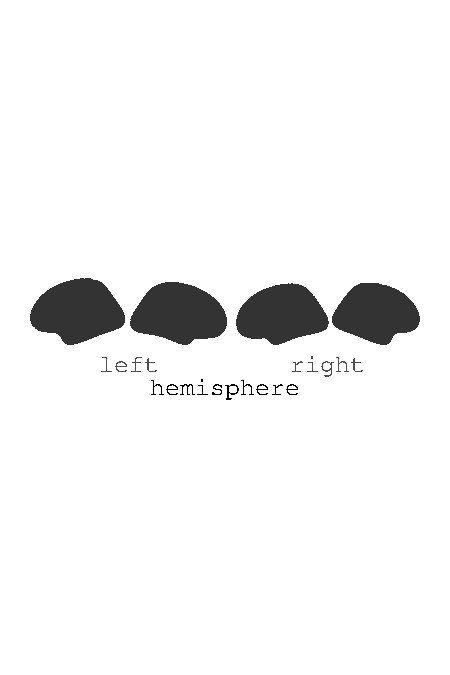
\includegraphics{msc_ggseg_files/figure-latex/figure1-1.pdf}
\caption{\label{fig:figure1}By default \texttt{ggseg()} will plot the dk atlas in grey shaded polygons.}
\end{figure}

In addition to the standard options for \emph{ggplot2} polygon geoms, the function also has several options for plotting the main brain representations.
These options are atlas-specific.
For cortical atlases, such as the \texttt{dk}, one can stack the hemispheres, display only the medial or lateral side, choose either one or both hemispheres, or any combination of hemisphere and view (see Figure \ref{fig:figure2} for examples).
For subcortical atlases, such as the \texttt{aseg} atlas, the options are more limited but one can often choose between axial, sagittal, and coronal views.



\begin{Shaded}
\begin{Highlighting}[]
\CommentTok{# A: dk dark theme}
\NormalTok{fig2A <-}\StringTok{ }\KeywordTok{ggseg}\NormalTok{(}\DataTypeTok{position =} \StringTok{"stacked"}\NormalTok{) }\OperatorTok{+}
\StringTok{  }\KeywordTok{theme_dark}\NormalTok{() }\OperatorTok{+}
\StringTok{  }\KeywordTok{labs}\NormalTok{(}\DataTypeTok{title=}\StringTok{"dk"}\NormalTok{, }\DataTypeTok{subtitle =} \StringTok{"dark theme"}\NormalTok{)}

\CommentTok{# B: dk medial view}
\NormalTok{fig2B <-}\StringTok{ }\KeywordTok{ggseg}\NormalTok{(}\DataTypeTok{view =} \StringTok{"medial"}\NormalTok{) }\OperatorTok{+}
\StringTok{  }\KeywordTok{labs}\NormalTok{(}\DataTypeTok{title =} \StringTok{"dk"}\NormalTok{, }\DataTypeTok{subtitle =} \StringTok{"medial view"}\NormalTok{)}

\CommentTok{# C: dk left medial alone}
\NormalTok{fig2C <-}\StringTok{ }\KeywordTok{ggseg}\NormalTok{(}\DataTypeTok{view =} \StringTok{"medial"}\NormalTok{,}
            \DataTypeTok{hemisphere =} \StringTok{"left"}\NormalTok{) }\OperatorTok{+}
\StringTok{  }\KeywordTok{labs}\NormalTok{(}\DataTypeTok{title=}\StringTok{"dk"}\NormalTok{, }\DataTypeTok{subtitle =} \StringTok{"medial left"}\NormalTok{)}

\CommentTok{# D: dk classic theme}
\NormalTok{fig2D <-}\StringTok{ }\KeywordTok{ggseg}\NormalTok{(}\DataTypeTok{position =} \StringTok{"stacked"}\NormalTok{) }\OperatorTok{+}
\StringTok{  }\KeywordTok{theme_classic}\NormalTok{() }\OperatorTok{+}
\StringTok{  }\KeywordTok{labs}\NormalTok{(}\DataTypeTok{title =} \StringTok{"dk"}\NormalTok{, }\DataTypeTok{subtitle =} \StringTok{"classic theme"}\NormalTok{)}


\CommentTok{# E: dk left hemisphere}
\NormalTok{fig2E <-}\StringTok{ }\KeywordTok{ggseg}\NormalTok{(}\DataTypeTok{hemisphere =} \StringTok{"left"}\NormalTok{) }\OperatorTok{+}
\StringTok{  }\KeywordTok{labs}\NormalTok{(}\DataTypeTok{title =} \StringTok{"dk"}\NormalTok{, }\DataTypeTok{subtitle =} \StringTok{"left hemisphere"}\NormalTok{)}

\CommentTok{# F: aseg default theme}
\NormalTok{fig2F <-}\StringTok{ }\KeywordTok{ggseg}\NormalTok{(}\DataTypeTok{atlas =}\NormalTok{ aseg, }\DataTypeTok{view =} \StringTok{"axial"}\NormalTok{) }\OperatorTok{+}
\StringTok{  }\KeywordTok{labs}\NormalTok{(}\DataTypeTok{title =} \StringTok{"aseg"}\NormalTok{, }\DataTypeTok{subtitle =} \StringTok{"axial view"}\NormalTok{)}

\CommentTok{# Using patchwork to combine all plots into one}
\NormalTok{(fig2A }\OperatorTok{|}\StringTok{ }\NormalTok{fig2B }\OperatorTok{|}\StringTok{ }\NormalTok{fig2C) }\OperatorTok{/}\StringTok{ }\NormalTok{(fig2D }\OperatorTok{|}\StringTok{ }\NormalTok{fig2E }\OperatorTok{|}\StringTok{ }\NormalTok{fig2F) }\OperatorTok{+}
\StringTok{  }\KeywordTok{plot_annotation}\NormalTok{(}\DataTypeTok{tag_levels =} \StringTok{'A'}\NormalTok{)}
\end{Highlighting}
\end{Shaded}

\begin{figure}[H]
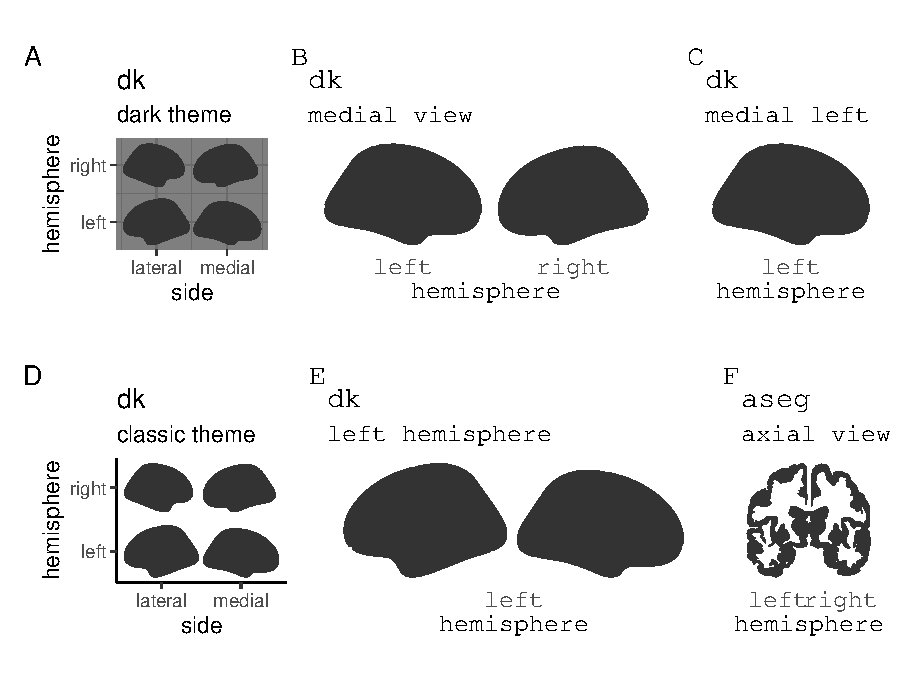
\includegraphics[width=1\linewidth]{msc_ggseg_files/figure-latex/figure2-1} \caption{\emph{ggseg} plots can be used with any \emph{ggplot2} feature such as standard scales and themes. For cortical atlases, one can supply special \emph{ggseg} options to determine, for example, hemisphere, view, or position. \textbf{A:} \texttt{dk} atlas, stacked with dark theme ; \textbf{B:} \texttt{dk} with medial view only; \textbf{C:} \texttt{dk} atlas with only left medial display; \textbf{D:} \texttt{dk} atlas, stacked, with classic theme; \textbf{E:} \texttt{dk} atlas with left hemisphere only; \textbf{F:} axial view of \texttt{aseg} atlas}\label{fig:figure2}
\end{figure}

\hypertarget{using-own-data-with-fill-and-colour}{%
\subsubsection{Using own data with fill and colour}\label{using-own-data-with-fill-and-colour}}

\texttt{ggseg()} accepts any argument you can supply to \texttt{geom\_polygon()}, and therefore is easy to work with for those familiar with \emph{ggplot2} functionality.
Standard arguments like \texttt{fill} that floods the segments with a colour, or \texttt{colour} that colours the edges around the segments are typical arguments to provide to the function either as a single setting value or within the \emph{ggplot2} mapping function \texttt{aes}.
To use color palettes corresponding to those used in the original neuroimaging softwares one can use atlas-specific `brain' palette scales (Figure \ref{fig:figure3}).



\begin{Shaded}
\begin{Highlighting}[]
\CommentTok{# Figure 3}
\KeywordTok{ggseg}\NormalTok{(}\DataTypeTok{mapping =} \KeywordTok{aes}\NormalTok{(}\DataTypeTok{fill =}\NormalTok{ region), }\DataTypeTok{colour=}\StringTok{"black"}\NormalTok{) }\OperatorTok{+}
\StringTok{  }\KeywordTok{scale_fill_brain}\NormalTok{(}\StringTok{"dk"}\NormalTok{) }\OperatorTok{+}
\StringTok{  }\KeywordTok{theme}\NormalTok{(}\DataTypeTok{legend.justification =} \KeywordTok{c}\NormalTok{(}\DecValTok{1}\NormalTok{,}\DecValTok{0}\NormalTok{),}
        \DataTypeTok{legend.position =} \StringTok{"bottom"}\NormalTok{,}
        \DataTypeTok{legend.text =} \KeywordTok{element_text}\NormalTok{(}\DataTypeTok{size =} \DecValTok{5}\NormalTok{)) }\OperatorTok{+}
\StringTok{  }\KeywordTok{guides}\NormalTok{(}\DataTypeTok{fill =} \KeywordTok{guide_legend}\NormalTok{(}\DataTypeTok{ncol =} \DecValTok{3}\NormalTok{))}
\end{Highlighting}
\end{Shaded}

\begin{figure}
\centering
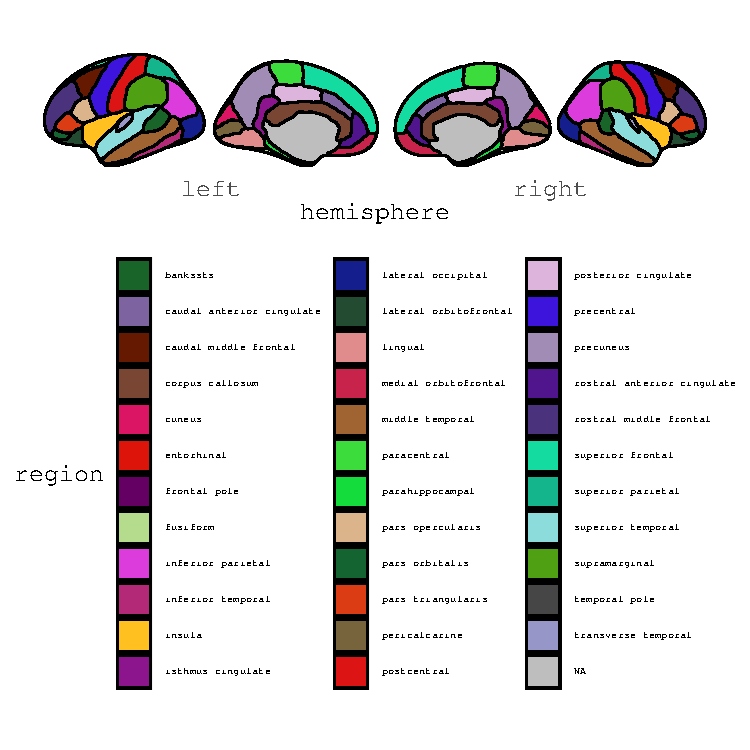
\includegraphics{msc_ggseg_files/figure-latex/figure3-1.pdf}
\caption{\label{fig:figure3}Supplying `region' to the fill option in \texttt{ggseg()}, will use the column `region' from the accompanying data-set to create a discrete colour palette over the segments in the atlas. The \texttt{dk} atlas default palette corresponds to the FreeSurferColorLut scheme.}
\end{figure}

Most users will use \texttt{ggseg()} to display - using a color scale - some descriptive or inferential statistics, such as mean thickness or brain-cognition relationships across the different brain regions.
Yet, before projecting the statistics onto the segments, one should explore the structure of the atlas data-sets.
The atlas data-set structure will help users understand what incoming statistical data needs to look like.
Note that each atlas corresponds to a unique data-set.
All data-sets have a similar structure and contain key information regarding the atlas, the region names, and the coordinates for the segment polygons.

\small

\begin{Shaded}
\begin{Highlighting}[]
\CommentTok{# Look at the top 5 rows of the dk data-set}
\KeywordTok{head}\NormalTok{(dk, }\DecValTok{5}\NormalTok{)}
\end{Highlighting}
\end{Shaded}

\normalsize

In any atlas, the column `label' is particularly useful for combining the data of interest with the \emph{ggseg}-polygons.
The column `label' contains the label (region) names as in the original neuroimaging software.
For example, the \texttt{dk} atlas label column matches the region names from Freesurfer statistics table outputs.
Yet, the data in \emph{ggseg} is in a long format - that is each region has a single row - and any data of interest needs to be in this same format.
Often data-sets are organized in wide format, in which subjects are represented by rows and each different data variable is represented in a separate column, and thus need to be rearranged to work with ggseg.
Summary statistic files from Freesurfer have a file format that can be difficult to work with in R.
In a set of functions in \emph{ggseg}, we facilitate conversion between FreeSurfer files and ggseg compatible data.
There is an \href{https://lcbc-uio.github.io/ggseg/articles/freesurfer_files.html}{extended vignette} of the various options.
In the following example, we import summary data that has been compiled using Freesurfer's \texttt{aparcstats2table} (for surfaces) or \texttt{asegstats2table} (volumes).
The summary files can combine parcellation metrics for one or more subjects into a single summary file.
This file also contains extra metrics like intracranial volume and total grey matter volume.
These later measures do not map onto ggseg, and as such, one should filter them out of the data returned from \texttt{read\_freesurfer\_table)}.

\small

\begin{Shaded}
\begin{Highlighting}[]
\NormalTok{file_path <-}\StringTok{ "data/aparc.volume.table"}

\NormalTok{someData <-}\StringTok{ }\KeywordTok{read_freesurfer_table}\NormalTok{(file_path, }\DataTypeTok{measure =} \StringTok{"volume"}\NormalTok{) }\OperatorTok\StringTok{ }
\StringTok{  }\CommentTok{# remove rows in the data that do not contain the strings "rh" or "lh"}
\StringTok{  }\NormalTok{dplyr}\OperatorTok{::}\KeywordTok{filter}\NormalTok{(}\KeywordTok{grepl}\NormalTok{(}\StringTok{"rh|lh"}\NormalTok{, label))}
\NormalTok{someData}
\CommentTok{## # A tibble: 34 x 3}
\CommentTok{##    subject label                      volume}
\CommentTok{##    <fct>   <chr>                       <dbl>}
\CommentTok{##  1 bert    rh_bankssts                  1969}
\CommentTok{##  2 bert    rh_caudalanteriorcingulate   2280}
\CommentTok{##  3 bert    rh_caudalmiddlefrontal       5390}
\CommentTok{##  4 bert    rh_cuneus                    2998}
\CommentTok{##  5 bert    rh_entorhinal                1735}
\CommentTok{##  6 bert    rh_fusiform                  8144}
\CommentTok{##  7 bert    rh_inferiorparietal         14876}
\CommentTok{##  8 bert    rh_inferiortemporal         11016}
\CommentTok{##  9 bert    rh_isthmuscingulate          1983}
\CommentTok{## 10 bert    rh_lateraloccipital         12729}
\CommentTok{## # ... with 24 more rows}
\end{Highlighting}
\end{Shaded}

\normalsize

A second option is to read in atlas files directly from the entire subject directory, using regular expression to select the target atlas.
The default aparc has a unique string ending with \texttt{aparc.stats} which we will use to read in all subject stats for that particular atlas.
One can filter specific subjects and/or regions from the R-object data.frame.

\begin{Shaded}
\begin{Highlighting}[]
\NormalTok{atlas_data <-}\StringTok{ }\KeywordTok{read_atlas_files}\NormalTok{(}
  \CommentTok{# Path to Freesurfers $SUBJECTS_DIR}
  \DataTypeTok{subjects_dir =} \StringTok{"/Applications/freesurfer/subjects/"}\NormalTok{,}
  \CommentTok{# Regular expression to find atlas files}
  \DataTypeTok{atlas =} \StringTok{"aparc.stats$"}
\NormalTok{)}
\NormalTok{atlas_data}
\CommentTok{## # A tibble: 204 x 11}
\CommentTok{##    subject label NumVert SurfArea GrayVol ThickAvg}
\CommentTok{##    <chr>   <chr>   <int>    <int>   <int>    <dbl>}
\CommentTok{##  1 bert    lh_b~    1181      831    2297     2.77}
\CommentTok{##  2 bert    lh_c~     843      572    1534     2.72}
\CommentTok{##  3 bert    lh_c~    2758     1840    5772     2.80}
\CommentTok{##  4 bert    lh_c~    2683     1654    3074     1.81}
\CommentTok{##  5 bert    lh_e~     581      416    1840     3.33}
\CommentTok{##  6 bert    lh_f~    4113     2875    8519     2.72}
\CommentTok{##  7 bert    lh_i~    4948     3466   10559     2.70}
\CommentTok{##  8 bert    lh_i~    5056     3542   12358     2.98}
\CommentTok{##  9 bert    lh_i~    1561      990    2350     2.09}
\CommentTok{## 10 bert    lh_l~    7961     5077   12743     2.30}
\CommentTok{## # ... with 194 more rows, and 5 more variables:}
\CommentTok{## #   ThickStd <dbl>, MeanCurv <dbl>,}
\CommentTok{## #   GausCurv <dbl>, FoldInd <int>, CurvInd <dbl>}
\end{Highlighting}
\end{Shaded}

This long format data can be used directly with the \texttt{ggseg()}-function, as the `label' column corresponds in name and content with the `label' column in the atlas data of \texttt{dk}.
The data \textbf{must} include a column that has the same column name and at least \emph{some} data matching the values in the corresponding column in the atlas data.
In the following example, the \texttt{ggseg()}-function will recognise the matching column `label', and merge the supplied data into the atlas using \emph{dplyr}-joins.
The appearance of the plot can then be modified similarly to any other \emph{ggplot2} graph using functions such as scales, labs, themes, etc., as seen in Figure \ref{fig:figure4}



\begin{Shaded}
\begin{Highlighting}[]

\CommentTok{# Figure 4A}
\NormalTok{fig4A <-}\StringTok{ }\NormalTok{someData }\OperatorTok\StringTok{ }
\StringTok{  }\CommentTok{# plot only subject bert}
\StringTok{  }\KeywordTok{filter}\NormalTok{(subject }\OperatorTok{==}\StringTok{ "bert"}\NormalTok{) }\OperatorTok\StringTok{ }
\StringTok{  }
\StringTok{  }\KeywordTok{ggseg}\NormalTok{(}\DataTypeTok{mapping=}\KeywordTok{aes}\NormalTok{(}\DataTypeTok{fill=}\NormalTok{volume))  }\OperatorTok{+}
\StringTok{  }\KeywordTok{labs}\NormalTok{(}\DataTypeTok{title=}\StringTok{"from read_freesurfer_table"}\NormalTok{, }
       \DataTypeTok{fill=}\StringTok{"volume}\CharTok{\textbackslash{}n}\StringTok{(mm^3)"}\NormalTok{) }\OperatorTok{+}
\StringTok{  }\KeywordTok{scale_fill_gradient}\NormalTok{(}\DataTypeTok{low=}\StringTok{"firebrick"}\NormalTok{,}\DataTypeTok{high=}\StringTok{"goldenrod"}\NormalTok{) }\OperatorTok{+}
\StringTok{  }\KeywordTok{guides}\NormalTok{(}\DataTypeTok{fill =} \KeywordTok{guide_colourbar}\NormalTok{(}\DataTypeTok{barheight =} \DecValTok{3}\NormalTok{))}

\CommentTok{# Figure 4B}
\NormalTok{fig4B <-}\StringTok{ }\NormalTok{atlas_data }\OperatorTok\StringTok{ }
\StringTok{  }\CommentTok{# plot only subject bert}
\StringTok{  }\KeywordTok{filter}\NormalTok{(subject }\OperatorTok{==}\StringTok{ "bert"}\NormalTok{) }\OperatorTok\StringTok{ }
\StringTok{  }
\StringTok{  }\KeywordTok{ggseg}\NormalTok{(}\DataTypeTok{mapping=}\KeywordTok{aes}\NormalTok{(}\DataTypeTok{fill=}\NormalTok{ThickAvg))  }\OperatorTok{+}
\StringTok{  }\KeywordTok{labs}\NormalTok{(}\DataTypeTok{title=}\StringTok{"from read_atlas_files"}\NormalTok{, }
       \DataTypeTok{fill=}\StringTok{"Thickness}\CharTok{\textbackslash{}n}\StringTok{(mean)"}\NormalTok{) }\OperatorTok{+}
\StringTok{  }\KeywordTok{scale_fill_gradient}\NormalTok{(}\DataTypeTok{low=}\StringTok{"forestgreen"}\NormalTok{,}\DataTypeTok{high=}\StringTok{"goldenrod"}\NormalTok{)}\OperatorTok{+}
\StringTok{  }\KeywordTok{guides}\NormalTok{(}\DataTypeTok{fill =} \KeywordTok{guide_colourbar}\NormalTok{(}\DataTypeTok{barheight =} \DecValTok{3}\NormalTok{))}

\NormalTok{(fig4A }\OperatorTok{/}\StringTok{ }\NormalTok{fig4B) }\OperatorTok{+}
\StringTok{  }\KeywordTok{plot_annotation}\NormalTok{(}\DataTypeTok{tag_levels =} \StringTok{"A"}\NormalTok{)}
\end{Highlighting}
\end{Shaded}

\begin{figure}
\centering
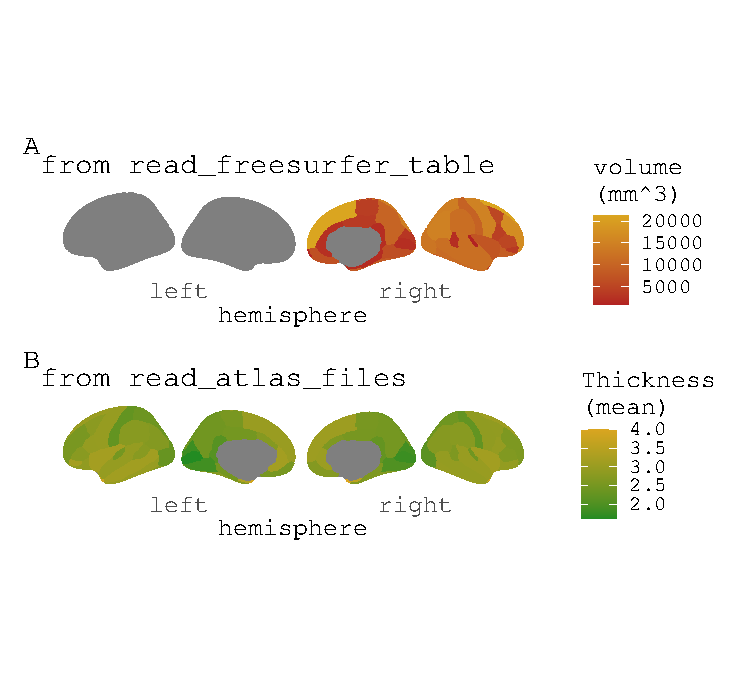
\includegraphics{msc_ggseg_files/figure-latex/figure4-1.pdf}
\caption{\label{fig:figure4}Supplying data through the `.data' option in \texttt{ggseg()} enables use of columns in the supplied data to aesthetical arguments (such as `fill'). The \emph{ggseg} plot can be used with any other polygon compatible function from \emph{ggplot2} or \emph{ggplot2} extentions, for instance adding title, changing the legend name and the colour scheme with standard \emph{ggplot2} functions.}
\end{figure}

If the results are only in one hemisphere, but you still want to plot both of them, make sure your data.frame includes the column `hemi' with either `right' or `left'.
In this case, data will be merged into the atlas both by `region' and by `hemi'.
For more information about adapting data and viewing only one hemisphere or side, the \href{https://lcbc-uio.github.io/ggseg/articles/ggseg.html\#single-hemisphere-results}{online documentation} contains more elaborate information.

\hypertarget{creating-subplots}{%
\subsubsection{Creating subplots}\label{creating-subplots}}

There is often the need to plot a statistic of interest in different groups (e.g.~thickness or brain - cognition relationships in young or older adults).
This may be obtained also with \texttt{ggseg()}, using \emph{ggplot2}'s \texttt{facet\_wrap} or \texttt{facet\_grid}, with three guiding rules:

\begin{enumerate}
\def\labelenumi{\arabic{enumi}.}
\tightlist
\item
  As before, data needs to be in long format with a column indexing which group the row corresponds to (group data should appear in separate rows, not in separate columns).\\
\item
  The data needs to be grouped using \emph{dplyr}'s \texttt{group\_by()} function \emph{before} providing the data to the \texttt{ggseg()}-function.
  The \texttt{ggseg()}-function will detect grouped data, and adapt it to \texttt{facet}'s requirements.\\
\item
  Apply \texttt{facet\_wrap} or \texttt{facet\_grid} to the plot having used the above two rules.
  An example of this can be seen in Figure \ref{fig:figure5} B, where a mock data-set including summary statistics for two groups (`Young' and `Old') is used when faceting a \emph{ggseg}-plot.
\end{enumerate}

The second rule is needed as the \texttt{ggseg()}-function is a ggplot-wrapper rather than an extension, and thus has a particular structure and pipeline to combine the atlas to supplied data.
The result of ungrouped data into \texttt{ggseg} is shown in \ref{fig:figure5} A.
Note that the data is combined incorrectly, there are three panels rather than two.
Regions not represented in the data (\texttt{NA}-values) have their own panel, while the remaining two panels only include regions with valid data.
All the concepts described above also work with the \texttt{aseg} atlas for subcortical structures, except for `hemisphere' and `view' arguments that are superfluous in subcortical atlases (Figure \ref{fig:figure6}).



\begin{Shaded}
\begin{Highlighting}[]
\CommentTok{# Make some simpler mock data}
\NormalTok{someData =}\StringTok{ }\KeywordTok{tibble}\NormalTok{(}
  \DataTypeTok{region =} \KeywordTok{rep}\NormalTok{(}\KeywordTok{c}\NormalTok{(}\StringTok{"transverse temporal"}\NormalTok{, }\StringTok{"insula"}\NormalTok{,}
               \StringTok{"precentral"}\NormalTok{,}\StringTok{"superior parietal"}\NormalTok{),}\DecValTok{2}\NormalTok{),}
  \DataTypeTok{p =} \KeywordTok{sample}\NormalTok{(}\KeywordTok{seq}\NormalTok{(}\DecValTok{0}\NormalTok{,.}\DecValTok{5}\NormalTok{,.}\DecValTok{001}\NormalTok{), }\DecValTok{8}\NormalTok{),}
  \DataTypeTok{AgeG =} \KeywordTok{c}\NormalTok{(}\KeywordTok{rep}\NormalTok{(}\StringTok{"Young"}\NormalTok{,}\DecValTok{4}\NormalTok{), }\KeywordTok{rep}\NormalTok{(}\StringTok{"Old"}\NormalTok{,}\DecValTok{4}\NormalTok{))}
\NormalTok{)}

\CommentTok{# Figure 5a}
\NormalTok{fig5A <-}\StringTok{ }\NormalTok{someData }\OperatorTok
\StringTok{  }\KeywordTok{ggseg}\NormalTok{(}\DataTypeTok{position =} \StringTok{"stacked"}\NormalTok{,}
      \DataTypeTok{mapping=}\KeywordTok{aes}\NormalTok{(}\DataTypeTok{fill=}\NormalTok{p), }\DataTypeTok{show.legend =} \OtherTok{FALSE}\NormalTok{) }\OperatorTok{+}
\StringTok{  }\KeywordTok{facet_wrap}\NormalTok{(}\OperatorTok{~}\NormalTok{AgeG, }\DataTypeTok{ncol=}\DecValTok{3}\NormalTok{) }\OperatorTok{+}
\StringTok{  }\KeywordTok{labs}\NormalTok{(}\DataTypeTok{title =} \StringTok{"Ungrouped data"}\NormalTok{)}

\CommentTok{# Figure 5b}
\NormalTok{fig5B <-}\StringTok{ }\NormalTok{someData }\OperatorTok
\StringTok{  }\KeywordTok{group_by}\NormalTok{(AgeG) }\OperatorTok
\StringTok{  }\KeywordTok{ggseg}\NormalTok{(}\DataTypeTok{position =} \StringTok{"stacked"}\NormalTok{,}
      \DataTypeTok{mapping=}\KeywordTok{aes}\NormalTok{(}\DataTypeTok{fill=}\NormalTok{p), }\DataTypeTok{show.legend =} \OtherTok{FALSE}\NormalTok{) }\OperatorTok{+}
\StringTok{  }\KeywordTok{facet_wrap}\NormalTok{(}\OperatorTok{~}\NormalTok{AgeG, }\DataTypeTok{ncol=}\DecValTok{3}\NormalTok{) }\OperatorTok{+}
\StringTok{  }\KeywordTok{labs}\NormalTok{(}\DataTypeTok{title =} \StringTok{"Grouped data"}\NormalTok{)}

\CommentTok{# Combining plots with patchwork, applying theme to all}
\NormalTok{(fig5A }\OperatorTok{/}\StringTok{ }\NormalTok{fig5B) }\OperatorTok{+}
\StringTok{  }\KeywordTok{plot_layout}\NormalTok{(}\DataTypeTok{widths =} \DecValTok{1}\NormalTok{) }\OperatorTok{+}\StringTok{ }
\StringTok{  }\KeywordTok{plot_annotation}\NormalTok{(}\DataTypeTok{tag_levels =} \StringTok{'A'}\NormalTok{) }\OperatorTok{&}
\StringTok{  }\KeywordTok{theme}\NormalTok{(}\DataTypeTok{axis.text =} \KeywordTok{element_text}\NormalTok{(}\DataTypeTok{size=}\DecValTok{8}\NormalTok{))}
\end{Highlighting}
\end{Shaded}

\begin{figure}[H]
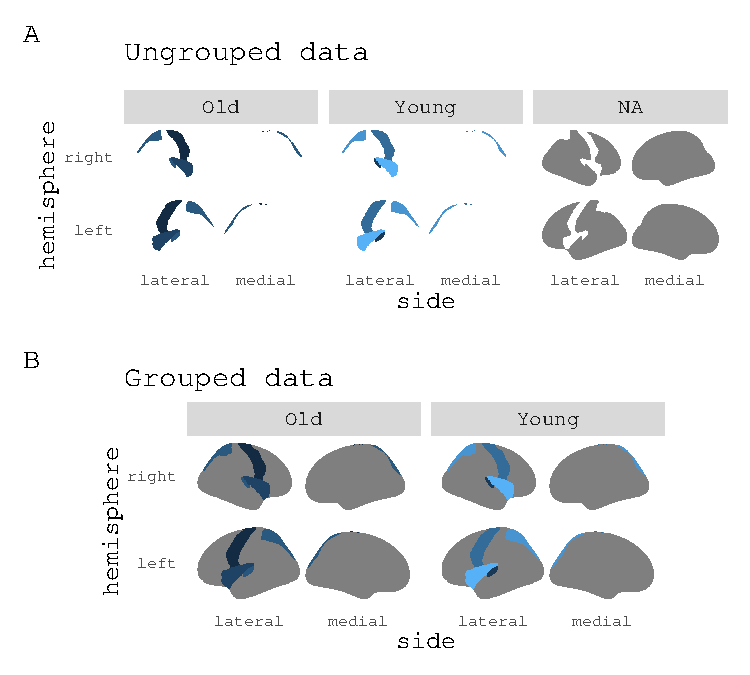
\includegraphics[width=1\linewidth]{msc_ggseg_files/figure-latex/figure5-1} \caption{Examples of incorrect and correct faceting with \texttt{ggseg}. \textbf{A}: ungrouped data will facet incorrectly due to the data not being merged correctly with the atlas. \textbf{B}: grouped data will merge in the expected way and result in correctly facetted plots.}\label{fig:figure5}
\end{figure}

The \texttt{ggseg} package also has extensive \href{https://lcbc-uio.github.io/ggseg/}{online documentation}, with more functionality than we have covered here.
The online documentation is also regularly updated with explanations of new features or code improvements.



\begin{Shaded}
\begin{Highlighting}[]
\CommentTok{# Figure 6}
\KeywordTok{ggseg}\NormalTok{(}\DataTypeTok{atlas=}\StringTok{"aseg"}\NormalTok{, }\DataTypeTok{mapping=}\KeywordTok{aes}\NormalTok{(}\DataTypeTok{fill=}\NormalTok{region)) }\OperatorTok{+}
\StringTok{  }\KeywordTok{theme}\NormalTok{(}\DataTypeTok{legend.justification=}\KeywordTok{c}\NormalTok{(}\DecValTok{1}\NormalTok{,}\DecValTok{0}\NormalTok{),}
        \DataTypeTok{legend.position=}\StringTok{"bottom"}\NormalTok{,}
        \DataTypeTok{legend.text =} \KeywordTok{element_text}\NormalTok{(}\DataTypeTok{size =} \DecValTok{5}\NormalTok{)) }\OperatorTok{+}
\StringTok{  }\KeywordTok{guides}\NormalTok{(}\DataTypeTok{fill =} \KeywordTok{guide_legend}\NormalTok{(}\DataTypeTok{ncol =} \DecValTok{3}\NormalTok{))}
\end{Highlighting}
\end{Shaded}

\begin{figure}
\centering
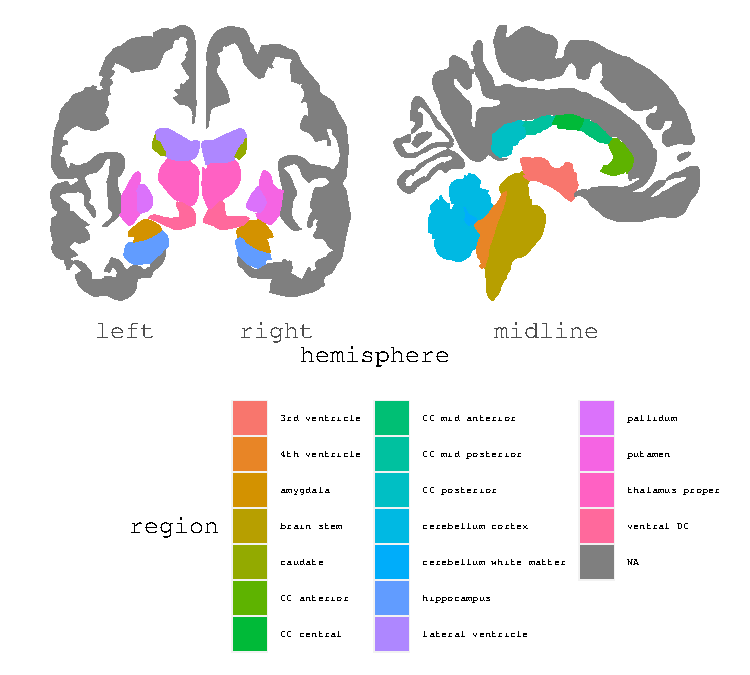
\includegraphics{msc_ggseg_files/figure-latex/figure6-1.pdf}
\caption{\label{fig:figure6}The \texttt{aseg} atlas showing subcortical structures has some distinct differences from the \texttt{dk}. For instance, there is no option to show only a single hemisphere. Furthermore, rather than showing lateral and medial surfaces, it shows an axial and sagittal slice.}
\end{figure}

\hypertarget{plotting-3d-mesh-data}{%
\subsection{Plotting 3D mesh data}\label{plotting-3d-mesh-data}}

Representing brains as 2D polygons is a good solution for fast, efficient, and flexible plotting, and can be easily combined with interactive apps such as Shiny (\citet{shiny}).
Yet, brains are intrinsically 3-dimensional and it can be challenging to recognize the location of a region as a flattened image.
This problem is exacerbated in atlases that represent subcortical features as they are 3-dimensional, while cortical structures, such as grey matter structures, can be flattened to 2-dimensions.
Hence, here we also provide the \emph{ggseg3d} package to plot, view, and print 3D-atlases in R.
\emph{ggseg3d} is based on tri-surface mesh plots using \emph{plotly} (\citet{plotly}).
The data structure is more complex than the \emph{ggplot2} polygons, and includes additional options for brain inflation, glass brains, camera locations, etc.
As \emph{ggseg3d} is based on plotly, the resulting brain atlases are interactive, which guides interpretation, and is useful for public dissemination.
We recommend users to familiarize themselves with \emph{plotly} (\citet{plotly}) when using this function.

Out-of-the-box, \texttt{ggseg3d()} plots the \texttt{dk\_3d} atlas in `LCBC' surface, but there are two more surfaces available for cortical atlases (Figure \ref{fig:figure7})
The `LCBC' surface consists on a semi-inflated white matter surface based on the \emph{fsaverage5} template subject, a surface template that is issued together with the \texttt{ggsegExtra} package.
All \texttt{{[}...{]}\_3d} atlases include a \texttt{colour} column that is based on the color scheme used in the source neuroimaging software.



\begin{Shaded}
\begin{Highlighting}[]
\CommentTok{# remotes::install_github("LCBC-UiO/ggseg3d")}
\KeywordTok{library}\NormalTok{(ggseg3d)}

\CommentTok{# Figure 7 left}
\NormalTok{fig7l <-}\StringTok{ }\KeywordTok{ggseg3d}\NormalTok{(}\DataTypeTok{surface =} \StringTok{"white"}\NormalTok{)  }\OperatorTok
\StringTok{  }\KeywordTok{pan_camera}\NormalTok{(}\StringTok{"right lateral"}\NormalTok{) }\OperatorTok
\StringTok{  }\KeywordTok{remove_axes}\NormalTok{() }\OperatorTok
\StringTok{  }\KeywordTok{layout}\NormalTok{(}\DataTypeTok{title=}\StringTok{"}\CharTok{\textbackslash{}n}\StringTok{ggseg3d(surface='white')"}\NormalTok{,}
         \DataTypeTok{font =}  \KeywordTok{list}\NormalTok{(}\DataTypeTok{size =} \DecValTok{30}\NormalTok{))}
\NormalTok{fig7l}

\CommentTok{# Figure 7 middle}
\NormalTok{fig7m <-}\StringTok{ }\KeywordTok{ggseg3d}\NormalTok{()  }\OperatorTok
\StringTok{  }\KeywordTok{pan_camera}\NormalTok{(}\StringTok{"right lateral"}\NormalTok{) }\OperatorTok
\StringTok{  }\KeywordTok{remove_axes}\NormalTok{() }\OperatorTok
\StringTok{  }\KeywordTok{layout}\NormalTok{(}\DataTypeTok{title=}\StringTok{"}\CharTok{\textbackslash{}n}\StringTok{ggseg3d(surface='LCBC')"}\NormalTok{,}
         \DataTypeTok{font =}  \KeywordTok{list}\NormalTok{(}\DataTypeTok{size =} \DecValTok{30}\NormalTok{))}
\NormalTok{fig7m}

\CommentTok{# Figure 7 right}
\NormalTok{fig7r <-}\StringTok{ }\KeywordTok{ggseg3d}\NormalTok{(}\DataTypeTok{surface =} \StringTok{"inflated"}\NormalTok{) }\OperatorTok
\StringTok{  }\KeywordTok{pan_camera}\NormalTok{(}\StringTok{"right lateral"}\NormalTok{) }\OperatorTok
\StringTok{  }\KeywordTok{remove_axes}\NormalTok{() }\OperatorTok
\StringTok{  }\KeywordTok{layout}\NormalTok{(}\DataTypeTok{title=}\StringTok{"}\CharTok{\textbackslash{}n}\StringTok{ggseg3d(surface='inflated')"}\NormalTok{,}
         \DataTypeTok{font =}  \KeywordTok{list}\NormalTok{(}\DataTypeTok{size =} \DecValTok{30}\NormalTok{))}
\NormalTok{fig7r}
\end{Highlighting}
\end{Shaded}

\begin{figure}[H]
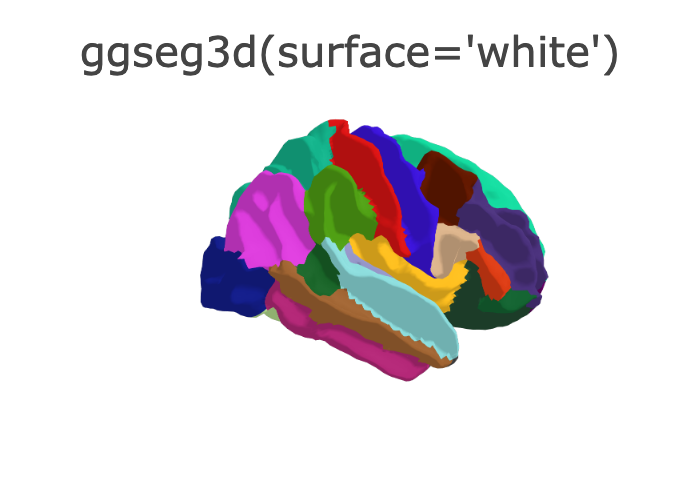
\includegraphics[width=0.3\linewidth]{msc_ggseg_files/figure-latex/figure7l} 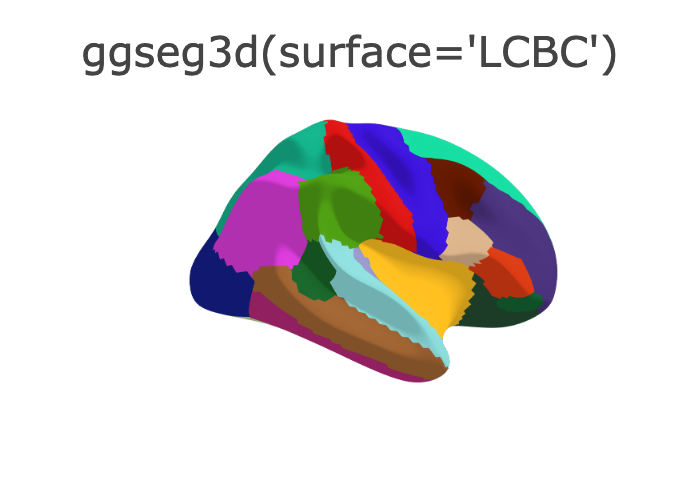
\includegraphics[width=0.3\linewidth]{msc_ggseg_files/figure-latex/figure7m} 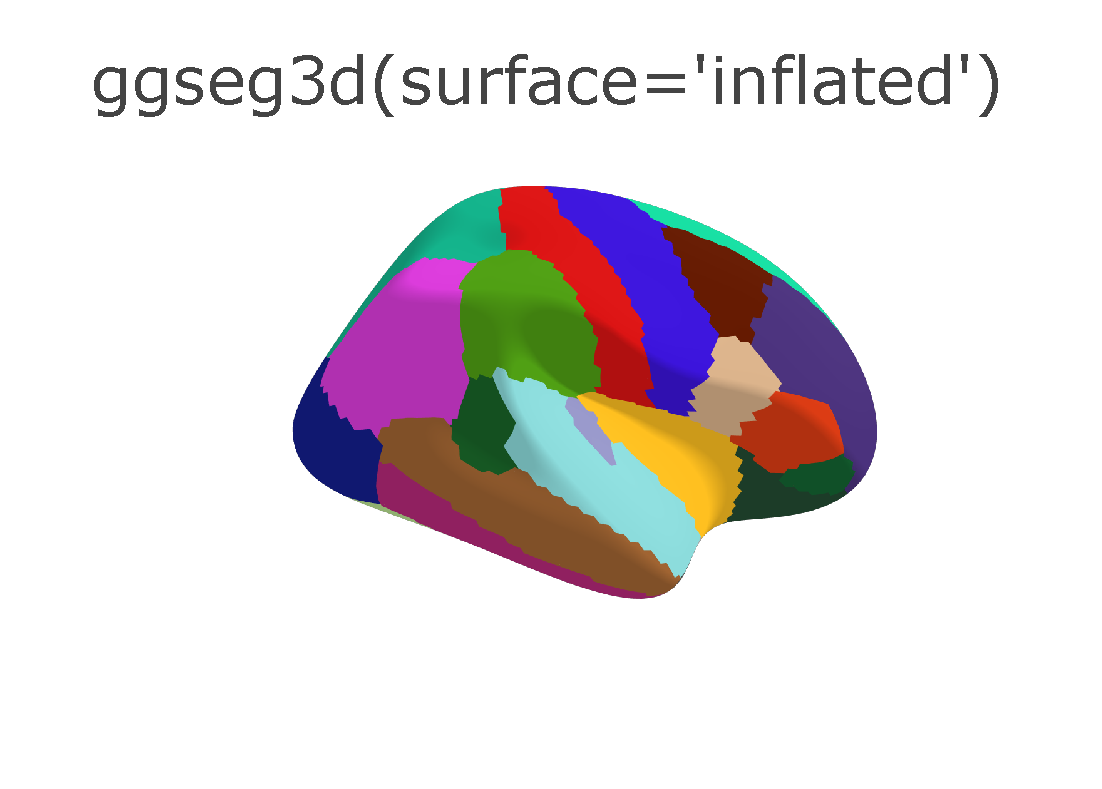
\includegraphics[width=0.3\linewidth]{msc_ggseg_files/figure-latex/figure7r} \caption{The three surface options provided in \emph{ggseg3d} atlases. \textbf{From left to right:} the `white' surface is the white matter surface, `LCBC' surface is the semi-inflated white matter surface (inflated over 10 iterations), and the `inflated' surface is a inflated grey matter cortical surface as provided by the FreeSurfer software. The title for each plot is the literal code use to make the subplot.}\label{fig:figure7}
\end{figure}

The 3D-atlas data is stored in nested tibbles.
Each cortical atlas has data-sets for three different surfaces (see Figure \ref{fig:figure7}) and the two hemispheres.
Only one surface is available for subcortical atlases as inflation procedures are irrelevant.
The `ggseg\_3d' column includes all necessary information for \texttt{ggseg3d()} to create a 3D mesh-plot, and should not be modified by the user.
The additional 3D-atlases in \emph{ggsegExtra} have the same data structure.
It is important to note that the coordinates in the plot (X, Y, Z) are \textbf{not} any type of radiological coordinate system, but arbitrary Cartesian plot coordinates.
While these coordinates are important when running imaging analyses and for reporting of the placement of these regions compared to other regions, this information is not preserved in \texttt{ggseg3d}, at the moment.
As such, information regarding referencing the regions' location in standard radiological spaces (like MNI or Taliarch) should be acquired directly from imaging software or papers describing the atlases, not \texttt{ggseg3d}.

\hypertarget{external-data-supply}{%
\subsubsection{External data supply}\label{external-data-supply}}

Similarly as in the 2D-atlas, the user will use \texttt{ggseg3d()} to display through a colour scale some descriptive or inferential statistic.
If the data is not already in the correct long format or uses similar naming as the atlas, the users should inspect the atlas data for a specific surface (and hemisphere, if desired), and then \texttt{unnest(ggseg\_3d)} it to see how the atlas data is organised.

\small

\begin{Shaded}
\begin{Highlighting}[]
\CommentTok{# Select surface and hemisphere, and then unnest to inspect the atlas data}
\NormalTok{dk_3d }\OperatorTok
\StringTok{  }\KeywordTok{filter}\NormalTok{(surf }\OperatorTok{==}\StringTok{ "inflated"} \OperatorTok{&}\StringTok{ }\NormalTok{hemi }\OperatorTok{==}\StringTok{ "right"}\NormalTok{) }\OperatorTok
\StringTok{  }\KeywordTok{unnest}\NormalTok{(ggseg_3d) }\OperatorTok
\StringTok{  }\KeywordTok{head}\NormalTok{(}\DecValTok{5}\NormalTok{)}
\CommentTok{## # A tibble: 5 x 9}
\CommentTok{##   atlas surf  hemi  region colour mesh  label}
\CommentTok{##   <chr> <chr> <chr> <chr>  <chr>  <lis> <chr>}
\CommentTok{## 1 dk_3d infl~ right <NA>   <NA>   <nam~ rh_u~}
\CommentTok{## 2 dk_3d infl~ right banks~ #1964~ <nam~ rh_b~}
\CommentTok{## 3 dk_3d infl~ right cauda~ #7D64~ <nam~ rh_c~}
\CommentTok{## 4 dk_3d infl~ right cauda~ #6419~ <nam~ rh_c~}
\CommentTok{## 5 dk_3d infl~ right corpu~ #7846~ <nam~ rh_c~}
\CommentTok{## # ... with 2 more variables: roi <chr>,}
\CommentTok{## #   annot <chr>}
\end{Highlighting}
\end{Shaded}

\normalsize

Note the \texttt{mesh} column, which contains lists.
Each list corresponds to a region and contains 6 vectors required to create the mesh of the tri-surface plot.
It should also be noted that the `label', `annot' and `region' columns could provide matching values for your own data.
Similarly to the \texttt{ggseg()}-function, the `label' column should match the region names used in the original neuroimaging software while `region' and `annot' provide alternative/secondary names.
It is thus important to match your regional identifiers with those used in the atlas.
To colour the segments using a column from the data, a column name from the data needs to be supplied to the \texttt{colour} option, and providing it to the \texttt{text} option will add another line to the \emph{plotly} hover information.



\begin{figure}[H]
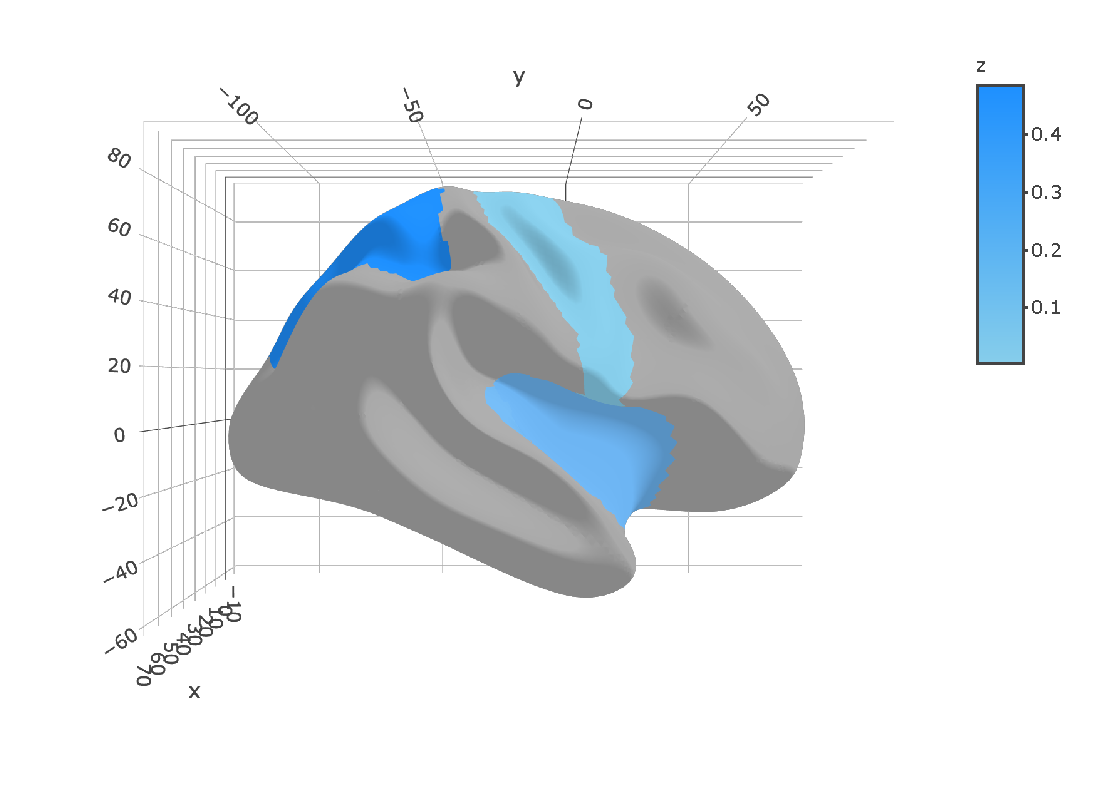
\includegraphics[width=0.3\linewidth]{msc_ggseg_files/figure-latex/figure8l} 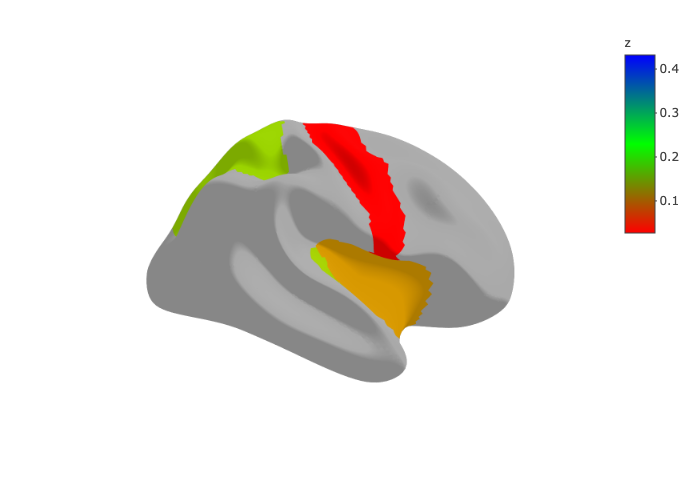
\includegraphics[width=0.3\linewidth]{msc_ggseg_files/figure-latex/figure8m} 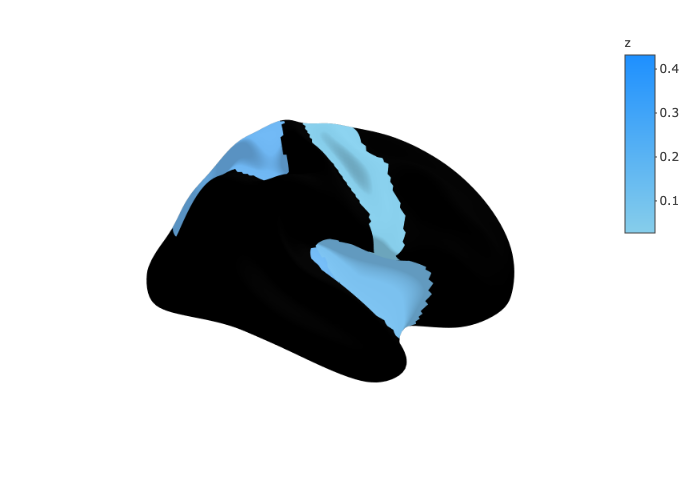
\includegraphics[width=0.3\linewidth]{msc_ggseg_files/figure-latex/figure8r} \caption{\textbf{Left:} Supplying data to \texttt{ggseg3d()} works similarly to \texttt{ggseg()}. Since \texttt{ggseg3d()} is based on \emph{plotly} rather than \emph{ggplot2}, most aesthetic adaptations must be set in the main function. Here we set the parcellation colours with the `colour' column and accompanying mouse-hover text with the `text' column. \textbf{Middle:} The palette for \emph{ggseg3d} needs to be specified directly in the main plot call. The `palette' option takes vectors of colours either as HEX-codes or R-colour names. \textbf{Right:} The colour of the \texttt{NA} values can also be changed through the option `na.colour'.}\label{fig:figure8}
\end{figure}

\hypertarget{customizing-colours-and-the-colour-bar}{%
\subsubsection{Customizing colours and the colour bar}\label{customizing-colours-and-the-colour-bar}}

You can provide custom colour palettes either in hex or R-names, as seen in Figure \ref{fig:figure8}.
Colours will be evenly spaced when creating the colour-scale.
A palette may also be supplied as a \emph{named numeric vector}, where the vector names are the colours that users wish to use, and the numeric values are the breakpoints for each colour (e.g. \texttt{c("red"\ =\ 0,\ "white"\ =\ 0.5,\ "blue"\ =\ 1)}).
This way the users can control the minimum and maximum values of the colour scale, and also how the gradient is applied.
If another colour than the default gray is wanted for the \texttt{NA} regions, supply `na.colour', either as HEX colour or colour name.
This option only takes a single colour.

\hypertarget{adding-a-glass-brain}{%
\subsubsection{Adding a glass brain}\label{adding-a-glass-brain}}

A glass brain is a translucent representation of the brain that can provide a frame of reference,
particularly when looking at subcortical parcellations and it only serves as a visual aid.
One can control the opacity of the these \texttt{NA} structures, to improve visualization, directly in the \texttt{ggseg3d} call.
A cortical glass brain can be added to \texttt{ggseg3d} plots through the function \texttt{add\_glassbrain()} (Figure \ref{fig:figure9}), which takes three extra arguments: hemisphere, colour, and opacity.
We recommend only using the glass brain function when plotting subcortical atlases.
A similar, interactive version of this plot can be found in the \href{https://lcbc-uio.github.io/ggseg3d//articles/ggseg3d.html\#colours-1}{online documentation}.

\begin{Shaded}
\begin{Highlighting}[]
\CommentTok{# Figure 9}
\NormalTok{fig9 <-}\StringTok{ }\KeywordTok{ggseg3d}\NormalTok{(}\DataTypeTok{atlas =}\NormalTok{ aseg_3d,}
        \DataTypeTok{na.alpha=} \FloatTok{.5}\NormalTok{) }\OperatorTok
\StringTok{  }\KeywordTok{add_glassbrain}\NormalTok{(}\StringTok{"left"}\NormalTok{) }\OperatorTok
\StringTok{  }\KeywordTok{pan_camera}\NormalTok{(}\StringTok{"left lateral"}\NormalTok{)}
\NormalTok{fig9}
\end{Highlighting}
\end{Shaded}



\begin{figure}[H]
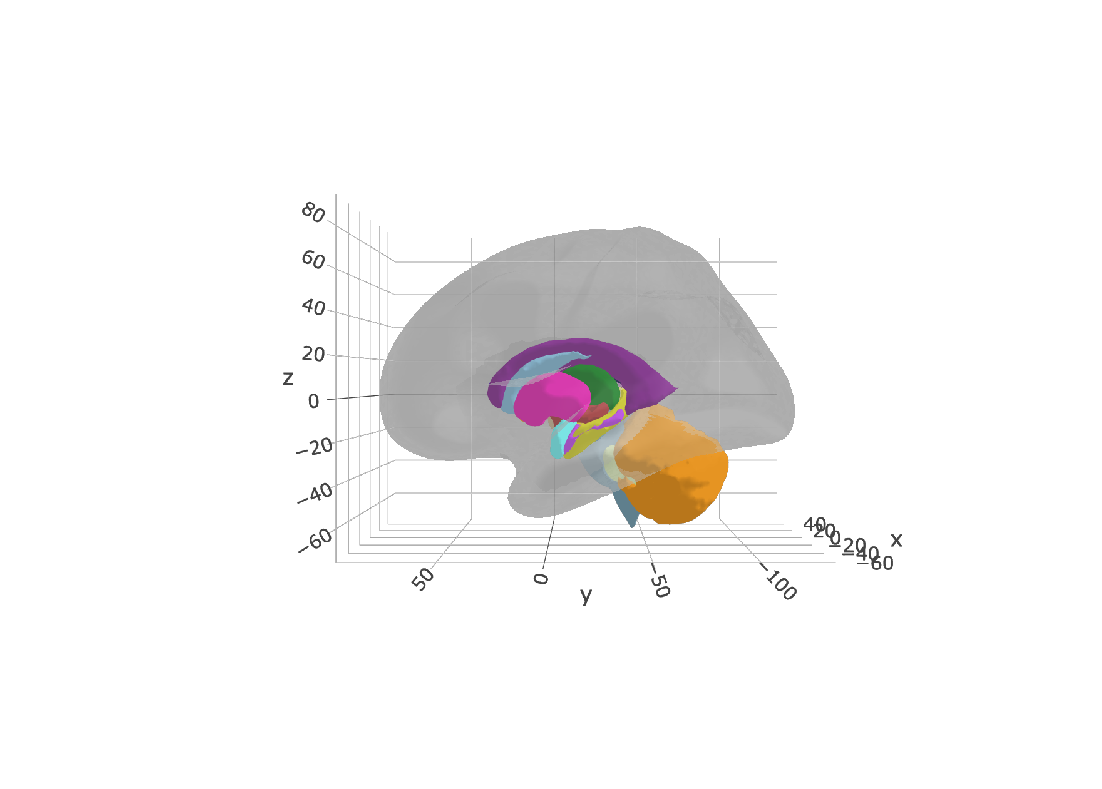
\includegraphics[width=0.6\linewidth]{msc_ggseg_files/figure-latex/figure9} \caption{For subcortical structure visualization, one can add a glass brain to the plot. This will help with locating the structures relative to the cortex, and make the plot easier to interpret. The glass brain is controlled by three options: opacity, hemisphere, and colour.}\label{fig:figure9}
\end{figure}

\texttt{ggsed3d()} is based on \emph{plotly} and thus additional \emph{plotly} functionalities can be used to modify and improve the 3D atlas representations.
In addition to Carson Sievert's book on \emph{plotly} in R (\citeyearpar{plotly}), we recommend resources for modifying axes in 3D plots (\citet{plotly-ax}), the basic introduction to tri-surface plots (\citet{plotly-tri}), and this tutorial on tri-surface plots with \emph{plotly} in R (\citet{plotly-trisurf}).
Finally, we recommend \href{https://github.com/plotly/orca\#installation}{orca} command line tool to save \emph{ggseg3d} atlas snapshots.

The package \href{https://lcbc-uio.github.io/ggseg3d/articles/ggseg3d.html}{online documentation} also includes interactive versions of many of the figures in this tutorial, and several more options not covered here.
The online documentation will also be updated as new features are required or we improve the current state of user functionality and options.

\hypertarget{additional-atlases}{%
\subsection{Additional atlases}\label{additional-atlases}}

The \emph{ggseg} and \emph{ggseg3d} packages have two atlases each, which are 2D and 3D variations of the same main atlases: the \texttt{dk} (\citet{dk}) and \texttt{aseg} (\citet{aseg}) atlases.
These are, however, only two among many meaningful ways of segmenting the brain into different regions.
Thus, the \emph{ggsegExtra} package is a library with two main functionalities: 1) to install additional data-sets for plotting with the \emph{ggseg} and \emph{ggseg3d} packages from other repositories, and 2) to create custom atlases for \emph{ggseg} and \emph{ggseg3d}.

\hypertarget{verified-existing-atlases}{%
\subsubsection{Verified existing atlases}\label{verified-existing-atlases}}

There is an ever-increasing amount of new atlases being created, as research and methods in neuroimaging analysis progresses.
The \emph{ggsegExtra}-package is intended to be expanded as a community-effort, as new and informative atlases are published.
A collection of the atlases currently listed in the \emph{ggsegExtra} package may be found in Figure \ref{fig:figure10} and explored in our \href{https://athanasiamo.shinyapps.io/ggsegDemo/}{shinyapps.io demonstration}.

\begin{Shaded}
\begin{Highlighting}[]
\CommentTok{# remotes::install_github("LCBC-UiO/ggsegExtra")}
\KeywordTok{library}\NormalTok{(ggsegExtra)}

\CommentTok{# list all known ggseg atlas-repositories}
\KeywordTok{ggseg_atlas_repos}\NormalTok{()}

\CommentTok{# list repositories matching a pattern search}
\NormalTok{yeo_repo <-}\StringTok{ }\KeywordTok{ggseg_atlas_repos}\NormalTok{(}\StringTok{"Yeo"}\NormalTok{)}
\CommentTok{## # A tibble: 10 x 5}
\CommentTok{##    repo       ggseg ggseg3d source comment        }
\CommentTok{##    <chr>      <lgl> <lgl>   <chr>  <chr>          }
\CommentTok{##  1 LCBC-UiO/~ TRUE  TRUE    github both 17 and 7 ~}
\CommentTok{##  2 LCBC-UiO/~ FALSE TRUE    github the 2009 atlas }
\CommentTok{##  3 LCBC-UiO/~ FALSE TRUE    github both thickness~}
\CommentTok{##  4 LCBC-UiO/~ FALSE TRUE    github both 17 and 7 ~}
\CommentTok{##  5 LCBC-UiO/~ TRUE  TRUE    github full atlas     }
\CommentTok{##  6 LCBC-UiO/~ TRUE  TRUE    github white tract at~}
\CommentTok{##  7 LCBC-UiO/~ TRUE  TRUE    github white tract at~}
\CommentTok{##  8 LCBC-UiO/~ FALSE TRUE    github white tract at~}
\CommentTok{##  9 LCBC-UiO/~ TRUE  FALSE   github Harvard-Oxford~}
\CommentTok{## 10 LCBC-UiO/~ TRUE  FALSE   github extra 2d view ~}
\end{Highlighting}
\end{Shaded}

Having found an existing atlas, you will need to install this like an R-library.
There is a convenience-function in \emph{ggsegExtra} that will help you do that.
Alternatively, you can install all the existing atlases.
This function will take time to execute and will consume quite some space as each atlas (particularly ggseg3d-atlases) can be large.
Once the atlases are installed, the atlas-packages can be loaded like any other R-package using \texttt{library}.

\begin{Shaded}
\begin{Highlighting}[]
\CommentTok{# Install ggseg-atlas listed by ggseg_atlas_repos("Yeo")}
\KeywordTok{install_ggseg_atlas}\NormalTok{(yeo_repo}\OperatorTok{$}\NormalTok{repo, yeo_repo}\OperatorTok{$}\NormalTok{source)}

\CommentTok{# This will take quite some time, there are many atlases with heavy data.}
\KeywordTok{install_ggseg_atlas_all}\NormalTok{()}
\end{Highlighting}
\end{Shaded}

\begin{Shaded}
\begin{Highlighting}[]
\KeywordTok{library}\NormalTok{(ggsegYeo2011)}
\KeywordTok{library}\NormalTok{(ggsegGlasser)}
\KeywordTok{library}\NormalTok{(ggsegDesterieux)}
\KeywordTok{library}\NormalTok{(ggsegICBM)}

\NormalTok{yeo7_p <-}\StringTok{ }\KeywordTok{ggseg}\NormalTok{(}\DataTypeTok{atlas =}\NormalTok{ yeo7 , }\DataTypeTok{mapping=}\KeywordTok{aes}\NormalTok{(}\DataTypeTok{fill=}\NormalTok{region),}
            \DataTypeTok{show.legend =} \OtherTok{FALSE}\NormalTok{, }\DataTypeTok{position=}\StringTok{"stacked"}\NormalTok{) }\OperatorTok{+}
\StringTok{  }\KeywordTok{scale_fill_brain}\NormalTok{(}\StringTok{"yeo7"}\NormalTok{, }\DataTypeTok{package =} \StringTok{"ggsegYeo2011"}\NormalTok{) }\OperatorTok{+}
\StringTok{  }\KeywordTok{labs}\NormalTok{(}\DataTypeTok{title=}\StringTok{"yeo7-data-set"}\NormalTok{)}

\NormalTok{glasser_p <-}\StringTok{ }\KeywordTok{ggseg}\NormalTok{(}\DataTypeTok{atlas =}\NormalTok{ glasser , }\DataTypeTok{mapping=}\KeywordTok{aes}\NormalTok{(}\DataTypeTok{fill=}\NormalTok{region),}
            \DataTypeTok{show.legend =} \OtherTok{FALSE}\NormalTok{, }\DataTypeTok{position=}\StringTok{"stacked"}\NormalTok{) }\OperatorTok{+}
\StringTok{  }\KeywordTok{scale_fill_brain}\NormalTok{(}\StringTok{"glasser"}\NormalTok{, }\DataTypeTok{package =} \StringTok{"ggsegExtra"}\NormalTok{) }\OperatorTok{+}
\StringTok{  }\KeywordTok{labs}\NormalTok{(}\DataTypeTok{title=}\StringTok{"glasser-data-set"}\NormalTok{)}

\NormalTok{ggsegs_p <-}\StringTok{ }\NormalTok{yeo7_p }\OperatorTok{+}\StringTok{ }\NormalTok{glasser_p }\OperatorTok{+}\StringTok{ }\KeywordTok{plot_annotation}\NormalTok{(}\DataTypeTok{tag_levels =} \StringTok{"A"}\NormalTok{)}

\NormalTok{desterieux_p <-}\StringTok{ }\KeywordTok{ggseg3d}\NormalTok{(}\DataTypeTok{atlas =}\NormalTok{ desterieux_3d) }\OperatorTok
\StringTok{  }\KeywordTok{pan_camera}\NormalTok{(}\StringTok{"right lateral"}\NormalTok{) }\OperatorTok
\StringTok{  }\KeywordTok{remove_axes}\NormalTok{() }\OperatorTok
\StringTok{  }\KeywordTok{add_annotations}\NormalTok{(}
    \DataTypeTok{text=}\StringTok{"desterieux_3d data-set"}\NormalTok{,}
    \DataTypeTok{y =} \DecValTok{1}\NormalTok{,}
    \DataTypeTok{yanchor =} \StringTok{'top'}\NormalTok{,}
    \DataTypeTok{legendtitle=}\OtherTok{TRUE}\NormalTok{, }\DataTypeTok{showarrow=}\OtherTok{FALSE}\NormalTok{,}
    \DataTypeTok{font =} \KeywordTok{list}\NormalTok{(}\DataTypeTok{family =} \StringTok{'sans serif'}\NormalTok{,}
                \DataTypeTok{size =} \DecValTok{50}\NormalTok{))}

\NormalTok{icbm_p <-}\StringTok{ }\KeywordTok{ggseg3d}\NormalTok{(}\DataTypeTok{atlas =}\NormalTok{ icbm_3d) }\OperatorTok
\StringTok{  }\KeywordTok{pan_camera}\NormalTok{(}\StringTok{"right lateral"}\NormalTok{) }\OperatorTok
\StringTok{  }\KeywordTok{add_glassbrain}\NormalTok{(}\StringTok{"left"}\NormalTok{) }\OperatorTok
\StringTok{  }\KeywordTok{remove_axes}\NormalTok{() }\OperatorTok
\StringTok{  }\KeywordTok{add_annotations}\NormalTok{(}
    \DataTypeTok{text=}\StringTok{"icbm_3d data-set"}\NormalTok{,}
    \DataTypeTok{y =} \DecValTok{1}\NormalTok{,}
    \DataTypeTok{yanchor =} \StringTok{'top'}\NormalTok{,}
    \DataTypeTok{legendtitle=}\OtherTok{TRUE}\NormalTok{, }\DataTypeTok{showarrow=}\OtherTok{FALSE}\NormalTok{,}
    \DataTypeTok{font =} \KeywordTok{list}\NormalTok{(}\DataTypeTok{family =} \StringTok{'sans serif'}\NormalTok{,}
                \DataTypeTok{size =} \DecValTok{50}\NormalTok{))}
\end{Highlighting}
\end{Shaded}



\begin{verbatim}
## Saving 6.5 x 4.5 in image
\end{verbatim}

\begin{figure}[H]
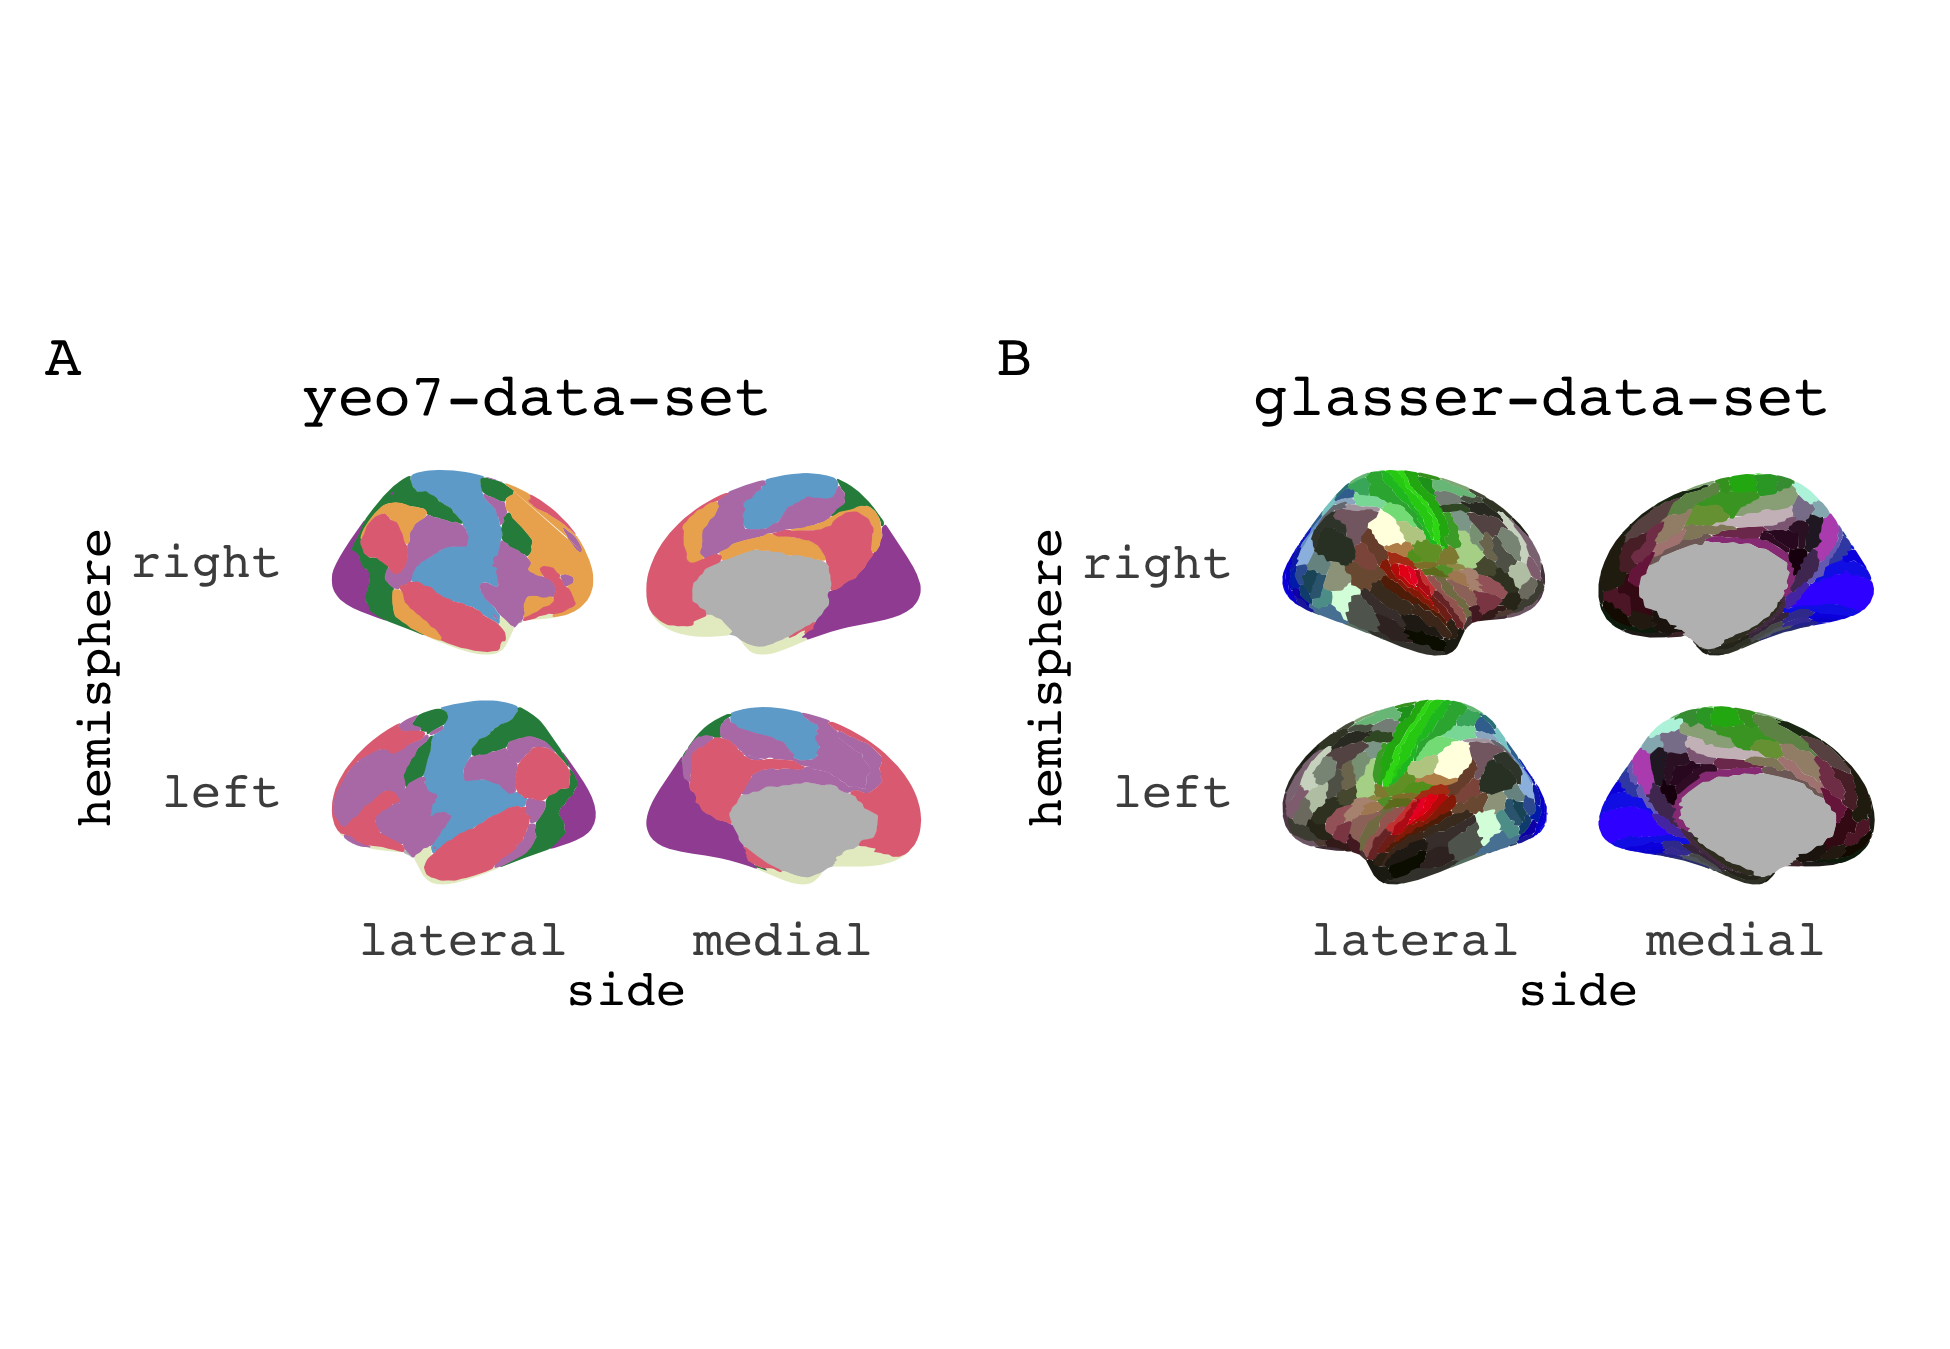
\includegraphics[width=0.8\linewidth]{msc_ggseg_files/figure-latex/figure10ab} 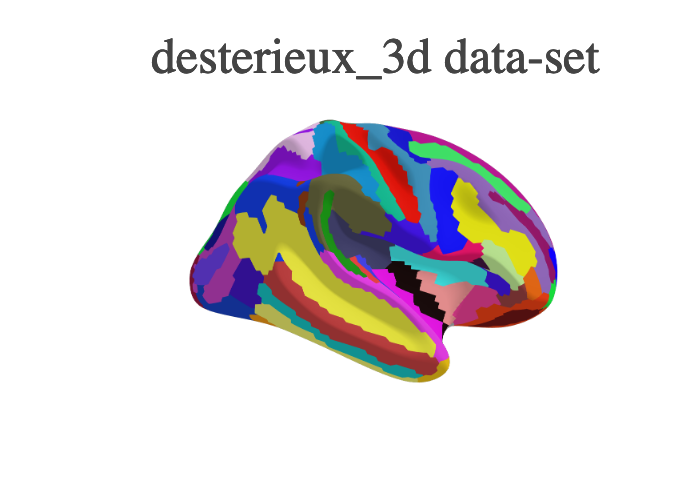
\includegraphics[width=0.4\linewidth]{msc_ggseg_files/figure-latex/figure10c} 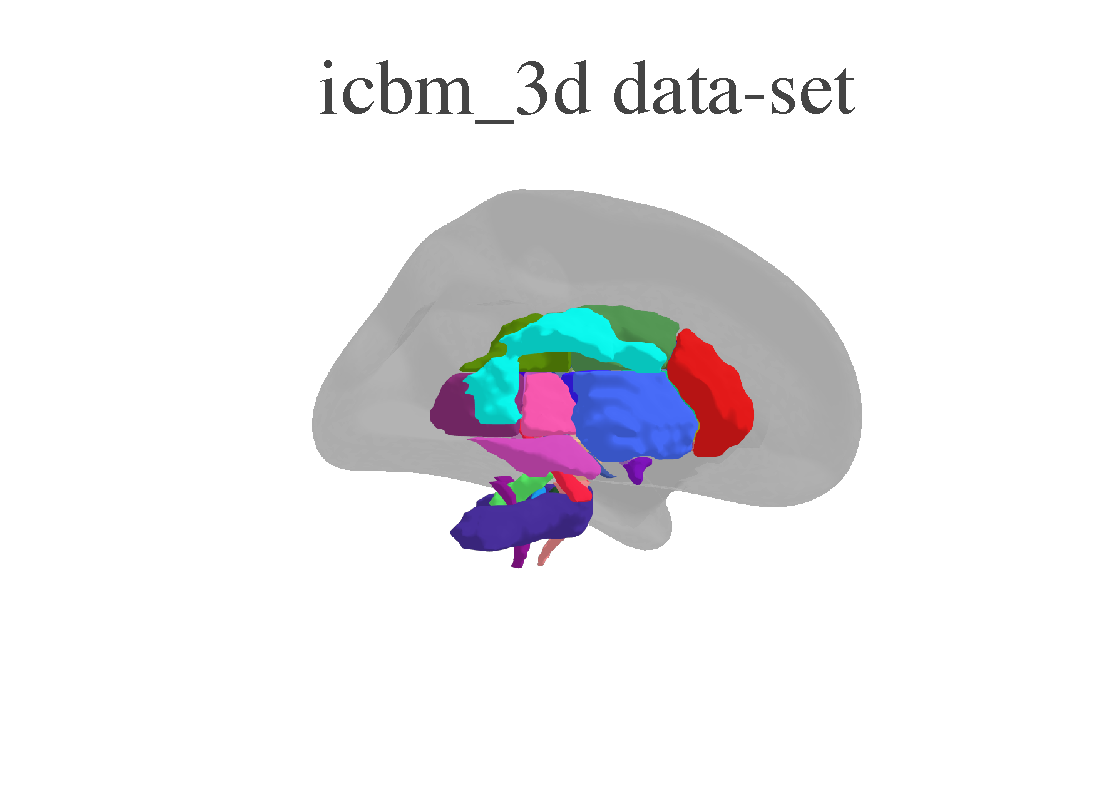
\includegraphics[width=0.4\linewidth]{msc_ggseg_files/figure-latex/figure10d} \caption{Four example data-sets from the \emph{ggsegExtra} library, plotted with the \texttt{ggseg()} and \texttt{ggseg3d()} functions.}\label{fig:figure10}
\end{figure}

\hypertarget{creating-custom-atlases}{%
\subsubsection{Creating custom atlases}\label{creating-custom-atlases}}

In many cases, users would like to create their own atlases based on existing parcellations or ones own imaging results.
There are several functions in \emph{ggsegExtra} to aid creating ones own atlas compatible with either \emph{ggseg} or \emph{ggseg3d}.
These processes depend on the origin of the segmentation (surface-based vs.~volume-based), and what type of system you are working on.
In addition, one will need other software dependencies to create new ggseg-compatible atlases.
Therefore, we will not describe the process here, but refer the readers to the ``Articles'' sections of the \href{https://lcbc-uio.github.io/ggsegExtra/index.html}{online documentation}, for further explanations and guides.
We encourage users who successfully create new atlases, to contribute to the \emph{ggsegExtra} brain atlas repository by adding the repository containing the brain atlases to the repository-list.

\hypertarget{discussion}{%
\section{Discussion}\label{discussion}}

The main aim of the \emph{ggseg}, \emph{ggseg3d}, and \emph{ggsegExtra} packages is to ease and streamline visualization of brain atlas data in R, by gathering a collection of atlases from several scientific sources and providing customized plotting functions.
In this tutorial, we introduced the packages to the readers by presenting some use examples and highlighting the main functions and options that are available.
As visualization tools, these packages add up to manifold functionalities such as ggBrain (\citet{ggBrain}) and ggneuro (\citet{ggneuro}) in R, and software-specific image viewers such as FSLeyes (\citet{fsleyes}) and Freeview (\citet{dale_99}).
In this regard, we do not aim to compete with software-specific visualizations or advocate for the superiority of the \emph{ggseg}-packages as visualization tools.
After all, flattened 2D polygons do not rely on a meaningful brain coordinate system and the units of information in 3D meshes are limited to the number of parcellations.
On the contrary, we believe the \emph{ggseg} niche among visualization tools resides in its simplicity and its ability to be combined with statistical analysis pipelines.
The possibility to serve as an interactive tool for dissemination and reproducibility when combined with other technologies, such as Binder (\citet{binder}) or Shiny (\citet{shiny}), is an added benefit.
This is exemplified in the \href{https://athanasiamo.shinyapps.io/Virtual_histology_2019/}{online supplementary information} of Vidal-Piñeiro et al. (\citeyearpar{vidal_2019}).

The functions in the \emph{ggseg}-packages provide users with the possibility of adapting the plots to their wishes, and also makes it possible to create and contribute to the atlas repository in \emph{ggsegExtra}.
The three \emph{ggseg}-packages contain three main features:

\begin{enumerate}
\def\labelenumi{\arabic{enumi}.}
\tightlist
\item
  A collection of 2D-polygon and 3D mesh brain parcellation atlases. The atlas data include the necessary coordinates for plotting, and include other information that should be recognizable for users.\\
\item
  \texttt{ggseg()} and \texttt{ggseg3d()} functions for visualization. Both functions are flexible and well-adapted to their environment and can be combined with any additional argument from \emph{ggplot2} and \emph{plotly}, respectively.
  \texttt{ggseg()} is a wrapper function for \texttt{geom\_polygon} from \emph{ggplot2} and it can be built upon like any \emph{ggplot2} object.
  \texttt{ggseg3d()} is a \emph{plotly} wrapper function for tri-surface mesh plots which prints 3D atlases.\\
\item
  Complimentary features, like color scales, and functions to convert compatible data frames to atlas-classes, read in likely data sources (like Freesurfer analysis output), and help create new atlases for use with \emph{ggseg} and \emph{ggseg3d}.
\end{enumerate}

The foundations of the \emph{ggseg}-packages trace back to the necessity of visualizing and exploring the lifespan trajectories of cortical thickness across different brain regions (see supplementary information in Vidal-Piñeiro et al. (\citeyearpar{vidal_2019}) ) .
That is, \emph{ggseg} appears with the need to inspect and display brain information over time - i.e.~including a spatial dimension and a time-varying factor - overcoming the constrains of printed journals and classical 2D plots (e.g.~bar plots).
The current state of science requires researches to share the results of studies in both high detail and in an intuitive manner, as it permits communication to wide audiences and facilitates reproducibility.
Hence, we believe this tool conforms to the essence of open science and invite users to improve the code, provide examples, or tutorials, and contribute to the atlas collection according to their own interest and needs via the public \href{https://github.com/LCBC-UiO/ggseg}{ggseg GitHub repository}, \href{https://github.com/LCBC-UiO/ggseg3d}{ggseg3d GitHub repository}, and \href{https://github.com/LCBC-UiO/ggsegExtra}{ggsegExtra GitHub repository}.

The ggseg-packages are based on \emph{ggplot2} and \emph{plotly}, which are only two of several visualisation tools in R, in addition to base-R plotting.
While the functionality presented here could also be integrated into packages such as \href{https://www.rdocumentation.org/packages/lattice/versions/0.20-40}{lattice}, both \emph{ggplot2} and \emph{plotly} have become established tools in the R-community and have extensive online documentation.
This makes them great packages to base further extensions and wrappers on.

Finally - while the \emph{ggseg}-packages are circumscribed to brain parcellations - we believe that the structure and functions of the package can be easily applied to any scientific field that benefits from data being displayed across the spatial dimension.
We encourage readers to borrow the package functionalities and adapt it to their respective fields and structures of interest, such as has already been done with the \emph{gganatogram}-package (\citet{gganatogram}).

\hypertarget{planned-package-improvements}{%
\section{Planned package improvements}\label{planned-package-improvements}}

In terms of planned \emph{ggseg} improvements, we are working on making a proper \texttt{geom} or \texttt{stat}.
While \texttt{ggseg()} works quite nicely as a \texttt{ggplot} wrapper, it introduces some unexpected work for the user, like having to group data \emph{before} faceting.
A \texttt{geom} or \texttt{stat} would benefit the user as it would behave more like other \emph{ggplot2} \texttt{geoms} and there would be less new functionalities to learn.

Concerning \emph{ggseg3d}, we also hope to make it possible to colour each individual mesh triangle, and as such provide the users with more flexibility in the plotting.
This should also improve the speed of \texttt{ggseg3d()}, which currently is quite slow due to each parcellation region being loaded into \texttt{plotly} sequentially.
Loading the entire brain mesh at once, and then coloring mesh triangles would significiantly improve the speed of \texttt{ggseg3d()}.
When able to colour the mesh triangles directly, rather than each parcellation individually, only full brain representations of each surface (rather than each surface of each atlas) needs to be stored, in addition to text data indexing mesh-locations.
This would reduce package size considerably, including package sizes of all atlas-repositories.

\hypertarget{conclusion}{%
\section{Conclusion}\label{conclusion}}

Visualization is a fundamental aspect of neuroimaging to explore and understand data, guide interpretation, and communicate with colleagues and the general audience.
In this tutorial, we have introduced the \emph{ggseg}-packages, tools for visualizing brain statistics through brain parcellation atlases in R.
This visualization tool easily combines with interactive routines as well as with diverse statistical analysis pipelines.
We hope this tool and tutorial proves useful to neuroscientists and inspires others to apply the functions in a wide variety of fields and structures.

\hypertarget{author-contributions}{%
\section{Author Contributions}\label{author-contributions}}

Didac Vidal-Piñeiro generated the idea for the tool, and the initial scripts for plot visualization.
He has also been responsible for converting images from neuroimaging data to ggseg-like data (e.g.~polygons and mesh data).
Athanasia M. Mowinckel adapted the initial scripts and made the functions into package format and has continued developing the functions with the aim of increasing user-friendliness.
She is also responsible for conceiving and adding the mesh-plot functionality through plotly, and developing the pipeline for making that possible.
A. M. Mowinckel wrote the first draft of the paper, and both have since critically edited it.

\hypertarget{conflicts-of-interest}{%
\section{Conflicts of Interest}\label{conflicts-of-interest}}

The authors declare that there were no conflicts of interest with respect to the authorship or the publication of this article.

\hypertarget{acknowledgements}{%
\section{Acknowledgements}\label{acknowledgements}}

We thank John Muschelli for package code comments and its adaptation to neuroconductor ({[}2018{]}), and Richard Beare for the first community created atlas, and base code comments.
We are indebted to A. M. Winkler scripts for converting neuroimaging data (Freesurfer) into .ply files, a necessary step for neuroimaging to mesh-plots conversion, and to Inge Amlien for the `LCBC' surface files and helpful contributions to the ggseg3d pipeline.
We are indebted to those users that actively contributed to the package and all the individuals that worked on the framework on which the package is sustained (e.g.~R-project, neuroimaging software).
Finally, we thank Anders M. Fjell (AMF) and Kristine B. Walhovd (KBW) for their encouragement and financial support.

\hypertarget{funding}{%
\section{Funding}\label{funding}}

This work is funded by EU Horizon 2020 Grant `Healthy minds 0-100 years: Optimizing the use of European brain imaging cohorts (Lifebrain)', with grant agreement 732592.
The project has also received funding from the European Research Council's Starting (grant agreements 283634, to A.M.F. and 313440 to K.B.W.) and consolidator Grant Scheme (grant agreement 771355 to KBW and 725025 to AMF).
The project has received funding through multiple grants from the Norwegian Research Council"

\hypertarget{prior-versions}{%
\section{Prior versions}\label{prior-versions}}

Some of the content presented here also appears in the package vignettes of \emph{ggseg} and \emph{ggseg3d}, which may be accessed through R or in the package websites (\citet{ggseg}, \citet{ggseg3d}).
Athanasia Monika Mowinckel also has several tutorials on her blog regarding \emph{ggseg} creation and functionality (\citet{ggsegAnim}, \citet{ggsegIntro}).

\renewcommand\refname{References}
\bibliography{references.bib}



\end{document}
